\chapter{Transferencia de carga en complejos nw de ZnO wurtzita + CAT.}
%\chapter{Fotodopaje de nw ZnO wurtzita con catecol}

El óxido de zinc (ZnO) es un material SC, compuesto por elementos de los grupos II-VI, de GAP amplio y directo ($3.37$ eV a temperatura ambiente) \cite{Strehlow1973}. En los últimos años ha generado un gran interés en la comunidad científica debido al gran número de aplicaciones prácticas que abarcan desde la pintura, la fotocatálisis hasta la medicina \cite{Djurisic2006,Mishra2017}. Las propiedades físicas del ZnO y su amplio GAP acoplado a la alta energía de enlace de excitones (60 meV) \cite{Ozgur2005} hace que sea un material adecuado para aplicaciones optoelectrónicas \cite{Janisch2005}, de esta manera, las nanoestructuras de ZnO también se emplean en el campo de la producción de energía fotovoltaica.

El ZnO puede cristalizar en estructura sal de roca, cúbica (blenda de zinc) o hexagonal (wurzita) (ver figura \ref{cristales_zno}), siendo esta última la más estable termodinámicamente en condiciones ambientales. Es un SC tipo n nativo debido a la desviación en la estequiometría que se origina a partir de las vacancias de oxígeno (V$_O$) y los átomos de zinc intersticial (Zn$_i$) \cite{Ozgur2005}. Los trabajos científicos de Look \emph{et al.} \cite{Look1998,Look1999} sostienen que el Zn$_i$ es el donante superficial nativo dominante en ZnO y otros proponen que la conductividad tipo n de las películas de ZnO dopadas involuntariamente se debe solo al hidrógeno \cite{Strzhemechny2004}. Esta suposición tiene sentido ya que el hidrógeno siempre está presente en todos los métodos de crecimiento y puede difundirse fácilmente en el ZnO en grandes cantidades debido a su gran movilidad. Cálculos de primeros principios basados en el DFT también sostienen que el hidrógeno incorporado involuntariamente actúa como una fuente de conductividad y se comporta como un donante superficial en ZnO \cite{VanDeWalle2000}. El dopaje de tipo n de ZnO es relativamente fácil en comparación con el dopaje de tipo p. Los elementos Al, Ga e In del grupo III como elementos sustitutos de Zn y los elementos Cl e I del grupo VII como elementos sustitutos de O pueden utilizarse como dopantes de tipo n \cite{Kato2002}. Sin embargo, es difícil alcanzar un buen dopaje tipo p en el ZnO debido a varias causas, una es la autocompensación causada por defectos intrínsecos, es decir, en un intento de dopar el material tipo p, ciertos defectos nativos que actúan como donantes pueden formarse espontáneamente y compensar deliberadamente aceptores \cite{Fan2013}, otra posibilidad es la baja solubilidad del dopante en el material. 


\begin{figure}[!htb]
\centering
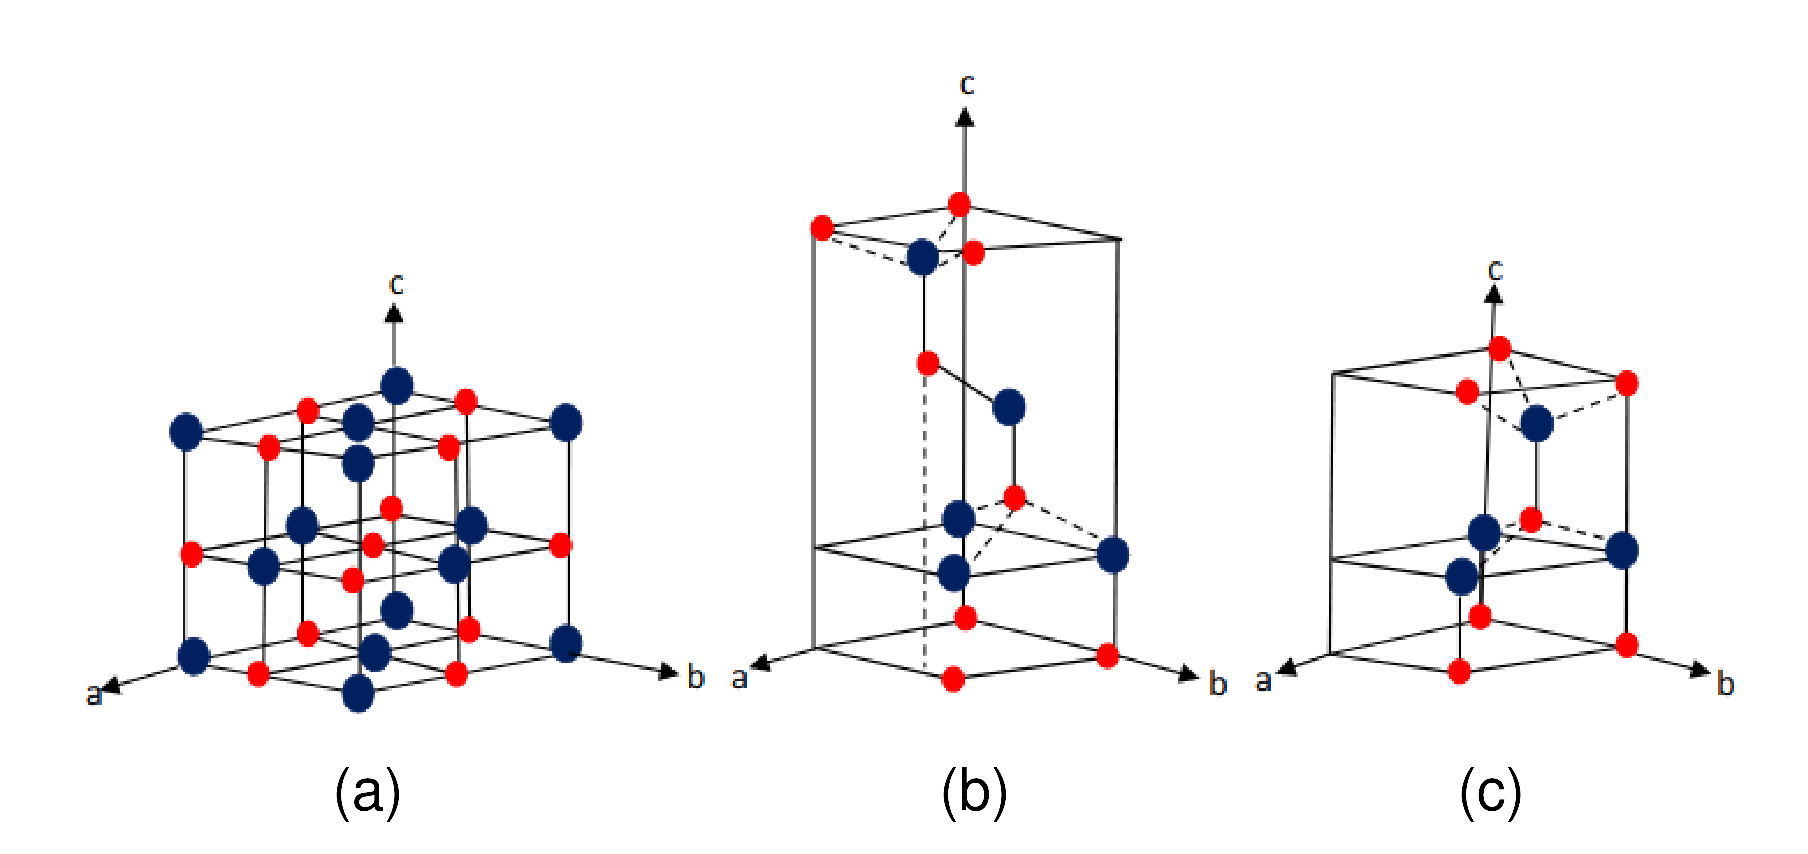
\includegraphics[height=5cm]{cap5/fig/est_zno.eps}
\caption{Estructuras cristalinas de ZnO: (a) sal de roca, (b) blenda de zinc y (c) wurtzita. Los círculos rojos y azules representan a los iones de zinc y oxígeno, respectivamente.} 
\label{cristales_zno}
\end{figure}

ZnO es un material amigable con el medio ambiente, en consecuencia, existe un interés en estudiar el ZnO en forma de polvos, monocristales, películas delgadas o nanoestructuras. Se han reportado una gran variedad de morfologías nanoestructuradas de ZnO como nanowires, nanorods, tetrapods, nanoribbons/belts, clusters \cite{Mishra2017, Huang2001_a,Huang2001_b, Liu2003,Shabani2020, Chauhan2018, Yan2003, Singh2020}, etc., como muestra la figura \ref{nanoestructuras_zno}. Los nanowires (nw) son SC unidimensionales que han captado la atención debido a sus propiedades físicas derivadas del confinamiento cuántico, como el transporte cuántico electrónico y la recombinación radiativa mejorada de portadores. Estas nanoestructuras son los sistemas ideales para estudiar los mecanismos de transporte en sistemas unidimensionales, que son beneficiosos no solo para comprender los fenómenos fundamentales en sistemas de baja dimensión sino también para desarrollar nanodispositivos de nueva generación con alto rendimiento \cite{Ozgur2005}. Los nw son prometedores en amplias aplicaciones y son los bloques de construcción fundamentales para la fabricación de nano-láseres de longitud de onda corta, transistores de efecto de campo, sensores ultrasensibles de gas de tamaño nanométrico, nanoresonadores, transductores, emisores de campo, etc. \cite{Huang2001_a,Wang2004_a, Wang2004_b,Heo2004}. De acuerdo a la literatura \cite{Ghosh2020,Nayeri2013,Peng2011,Baxter2005}, los nw de ZnO wurtzita también son buenos candidatos para fotoelectrodos en las DSSC, no solo por las ventajas de la morfología, al proporcionar una ruta directa a los electrones, sino también por las propiedades que provienen del material como la alta movilidad electrónica con respecto a otros SC, crecimiento anisotrópico, la facilidad de cristalización, etc. \cite{Tiwana2011,Law2005} que también aportan al buen funcionamiento de la celda.

\begin{figure}[!htb]
\centering
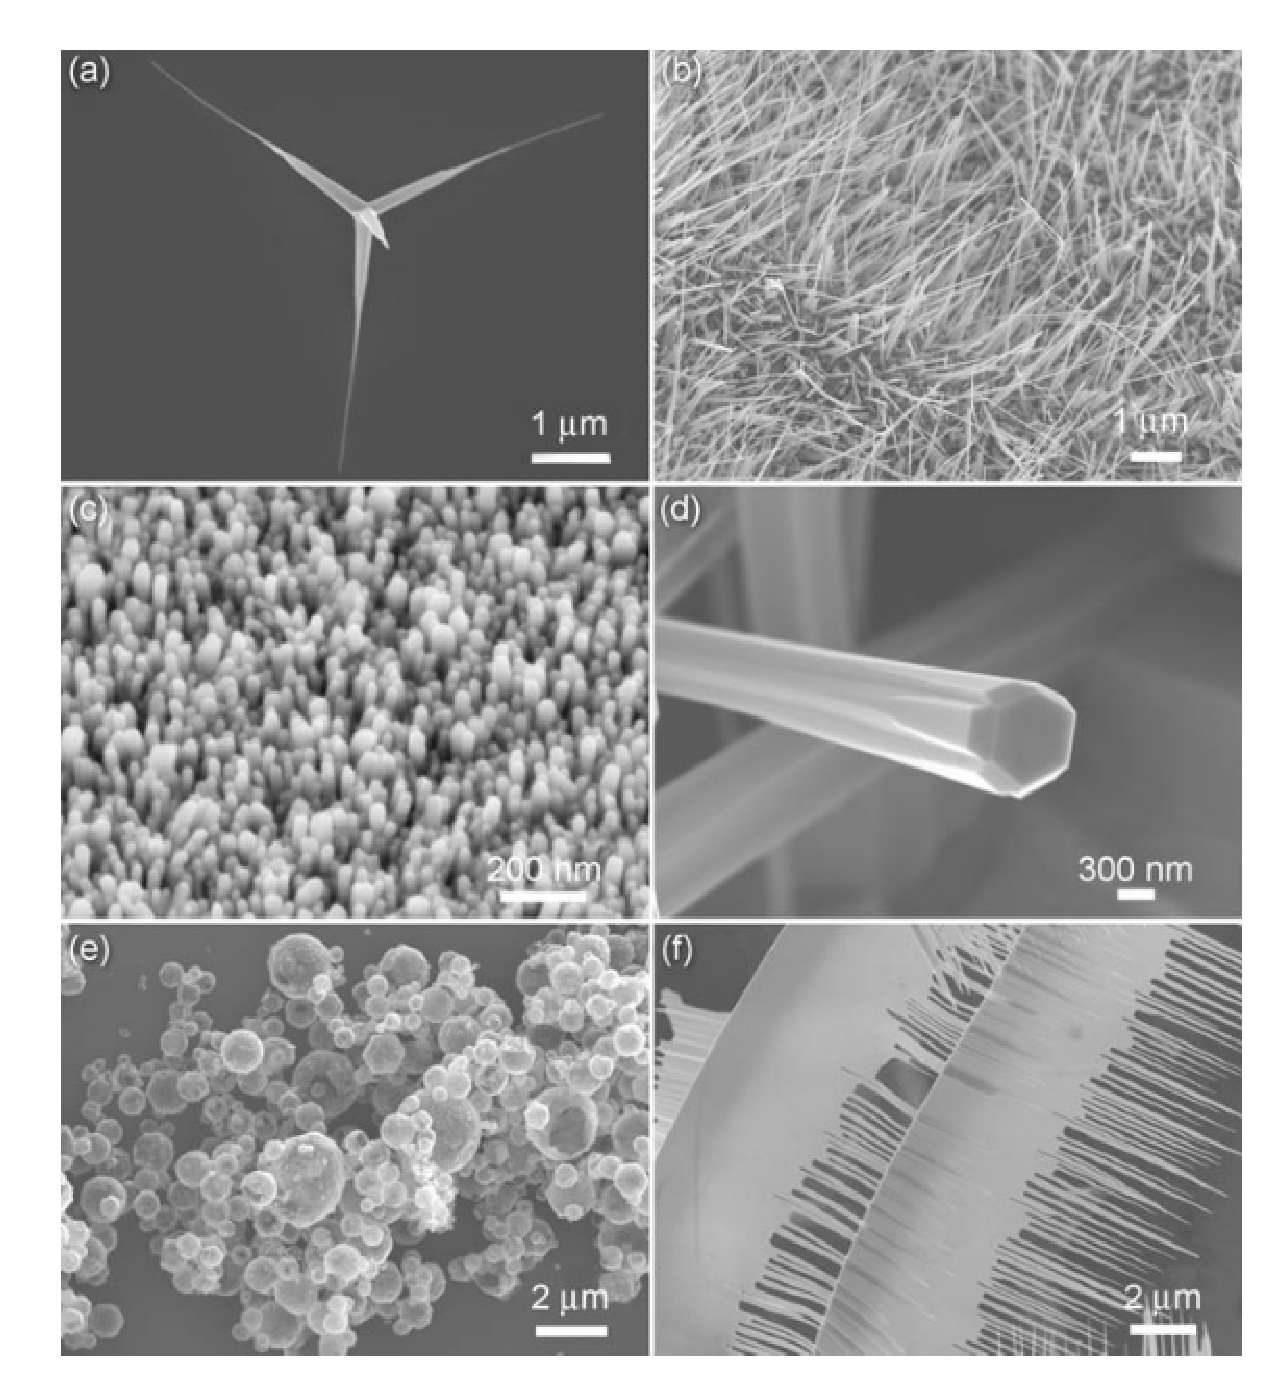
\includegraphics[height=9cm]{cap5/fig/nanoestructuras_zno.eps}
\caption{ (a-f) Imágenes representativas de microscopía electrónica de barrido de diversas morfologías de nanoestructura de ZnO. Extraído de \cite{Djurisic2006}}
\label{nanoestructuras_zno}
\end{figure}

Como se mencionó en el capítulo 4, las DSSC se clasifican en tipo I y tipo II  dependiendo de la vía de inyección que tomen los electrones desde el colorante absorbido al SC (ver figura \ref{tipos_dssc}). En las celdas tipo II, los electrones se inyectan no sólo por el camino indirecto o tipo I, sino también por la vía directa o de “un sólo paso” desde el estado fundamental del sensibilizador a la BC del SC mediante la excitación fotoinducida de las bandas de transferencia de carga colorante-SC ({\bf C-S}) como se ilustra en el esquema (b) de la figura \ref{tipos_dssc}. 

\begin{figure}[!htb]
\centering
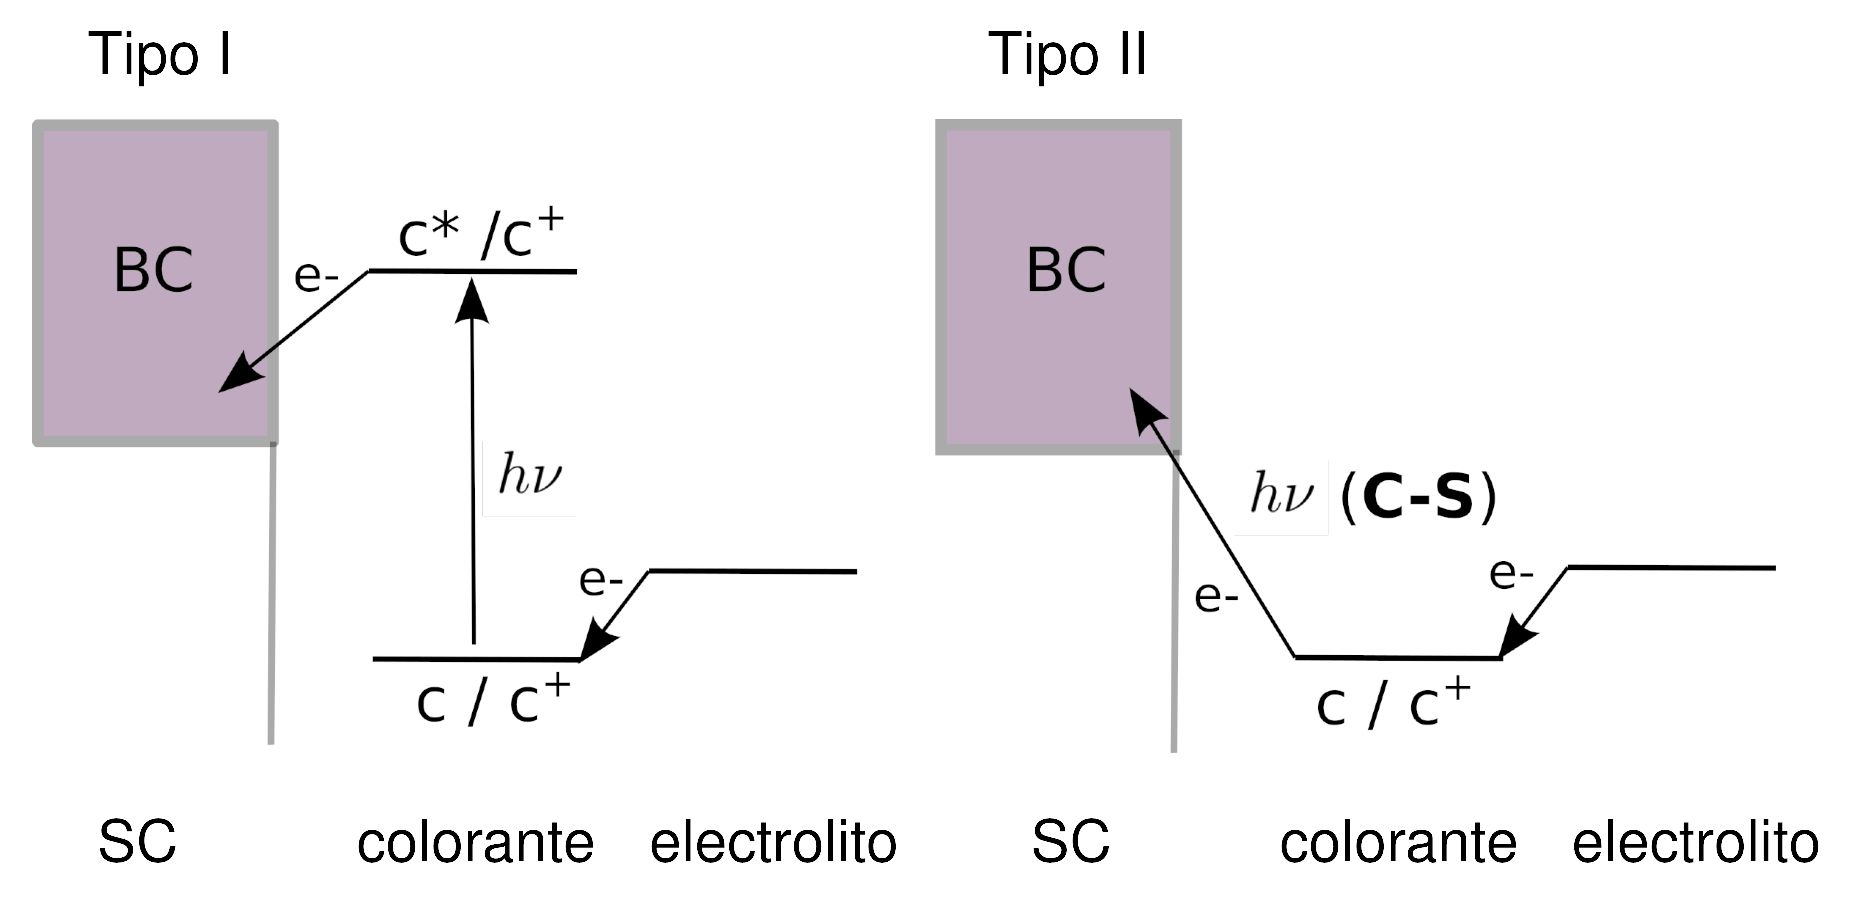
\includegraphics[height=7cm]{cap5/fig/tipo1_tipo2.eps}
\caption{Diferentes vías de inyección electrónica en sistemas colorante-SC desde la molécula al SC}
\label{tipos_dssc}
\end{figure}

De trabajos anteriores se conoce que las moléculas que tienen enodiol en su estructura se unen a la superficie del TiO$_2$ a través de la quelación de los iones de Ti de la superficie con los grupos enodiol, dando lugar a bandas de C-S generalmente muy intensas \cite{Tae2005}. En particular, el CAT y sus derivados como la dopamina, fluorona, numerosos pigmentos naturales como el rojo de bromopirogalol y las antocianinas \cite{Sinopoli2017, Persson2000, Dimitrijevic2003, Frei1990, Ramakrishna2001} son ejemplos típicos de DSSC de tipo II ya que tienen restos de CAT en su estructura y en consecuencia muestran fuertes bandas C-S en la región visible al unirse al TiO$_2$. También se ha demostrado que la fotoexcitación de las bandas C-S da lugar a una inyección directa de electrones de los colorantes al TiO$_2$ muy rápida, menor a $100$ fs \cite{Wang2003,Huber2000}, de acuerdo con la teoría de transferencia de carga de Mulliken \cite{Mulliken1952}.

A pesar de que los colorantes tipo II puedan inyectar electrones al TiO$_2$ por dos caminos y la eficiencia de inyección de electrones de la vía directa, en principio debería ser 1, no se han empleado rigurosamente como sensibilizadores para DSSC debido a que los valores de eficiencia cuántica externa ({\bf EQE}) son menores a las eficiencias de las DSSC sensibilizadas con colorantes tipo I. Una de las razones por las que la EQE de la vía directa son tan bajas radica en el hecho de que las velocidades de transferencia electrónica desde el TiO$_2$ reducido a la molécula oxidada, es decir la recombinación de carga, son mayores para la vía directa (en el orden de los picosegundos \cite{Ramakrishna2001,Wang2003, Huber2000}) que para la indirecta. En este sentido, el desarrollo de métodos para aumentar la eficiencia de la vía directa no es solo un gran desafío en sí mismo sino que también de gran interés desde el punto de vista académico y práctico.

En el capítulo previo, se estudió el complejo CAT-NP TiO$_2$ no solo porque es un colorante que opera por la vía directa sino también porque cuando se adsorbe sobre la superficie de TiO$_2$, el umbral de absorción óptica se reduce significativamente en energía. Como muestra la figura \ref{specs_cat}, la cual expone los espectros de absorción óptica del catecol aislado obtenido experimentalmente \cite{Dewar1958} y calculado con dftb+, el máximo de absorción de la banda de mínima energía se encuentra en la zona del UV. Ambos espectros son similares cualitativamente, teniendo en cuenta que en el espectro experimental se utilizó un solvente orgánico en la medición mientras que en el cálculo teórico el CAT se encuentra en el vacío. 

En este capítulo se realizaron estudios teóricos a nivel DFTB y TD-DFTB de la estructura electrónica y propiedades ópticas de los complejos {\bf CAT-nw ZnO} debido a las particularidades que presentan el CAT y el nw desde el punto de vista electrónico aunque a priori no sea un sistema que garantice una buena eficiencia en una DSSC al tratar con un sensibilizador tipo II. 

\begin{figure}[!htb]
\centering
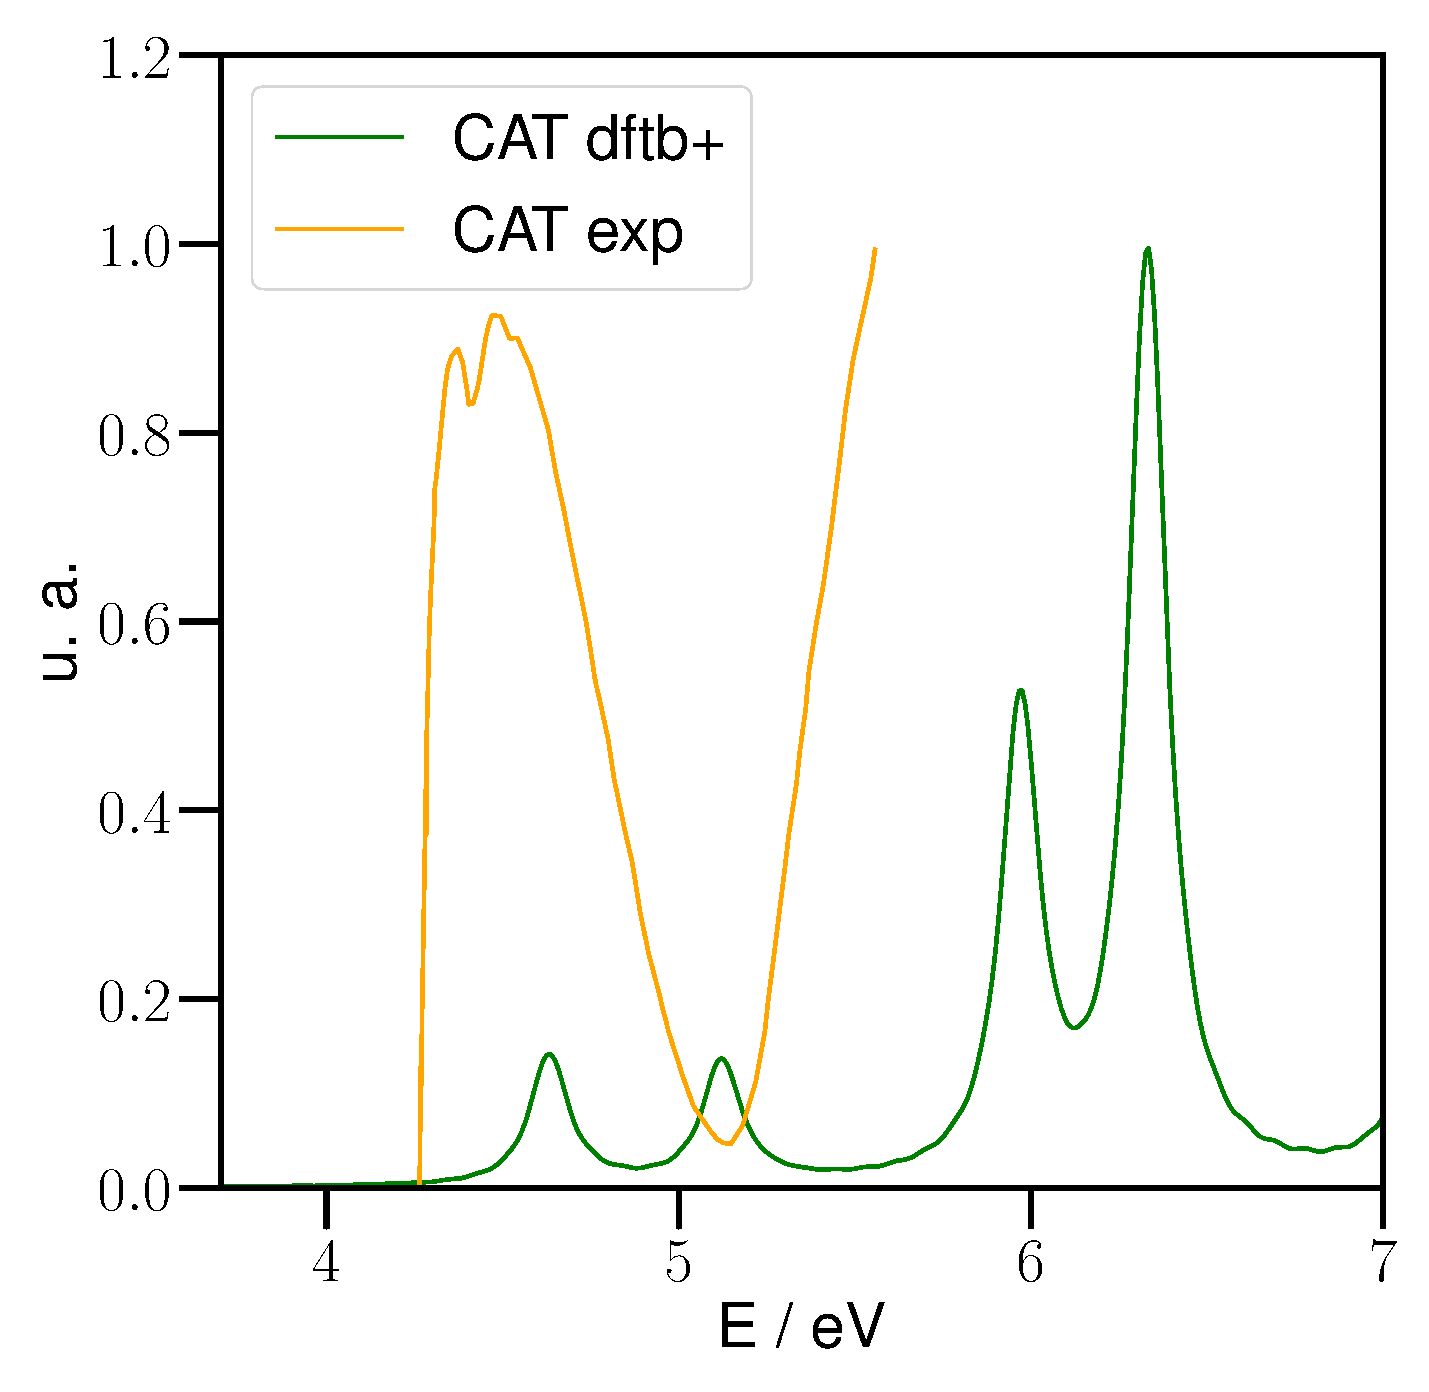
\includegraphics[height=9cm]{cap5/fig/specs_cat.eps}
\caption{Espectros de absorción óptica de CAT aislado obtenidos experimentalmente (naranja) y teóricamente con dftb+ (verde)}
\label{specs_cat}
\end{figure}

\section{Detalles computacionales}

Los parámetros utilizados para calcular los espectros de absorción y las dinámicas electrónicas son los mismos que se utilizaron en el capítulo 4, es decir: paso de tiempo $0.005$ fs, cantidad de pasos 20000 e intensidad del campo $0.0001$ $\frac{V}{\AA}$ y $0.01$ $\frac{V}{\AA}$, respectivamente. La diferencia radica en el estudio de la dinámica electrónica del sistema analizado, ya que en este capítulo se realizó aplicando perturbaciones sinusoidales sintonizadas con la energía de los máximos de absorción en el rango (0-4) eV.

\section{Estructura electrónica en equilibrio}

\subsection{Energía de adsorción}


\begin{figure}[!htb]
\centering
\includegraphics[height=4.5cm]{cap5/fig/estructuras_flecha.eps}
\caption{Sistemas de estudio CAT+nw con diferentes cubrimientos. Con colores más intensos se muestra la celda unidad (C$_1$) y las superceldas (el resto de los complejos)}
\label{estructuras}
\end{figure}


El primer objetivo del capítulo fue estudiar los distintos cubrimientos de colorante (CAT) en el nw (ver figura \ref{estructuras}) y analizar el efecto que produce en la estructura electrónica en el equilibrio. Para realizar el estudio se utilizaron 6 sistemas CAT-nw: {\bf C$_1$}, {\bf C$_2$}, {\bf C$_3$}, {\bf C$_4$}, {\bf C$_5$} y {\bf C$_6$}, los cuales son el resultado de la adsorción monodentada del colorante en su forma disociada a la superficie del nw. En trabajos anteriores del grupo \cite{Negre2012} hemos encontrado que aunque la unión bidentada disociativa del CAT es energéticamente preferida, para este modelo de TB, esta forma es inestable y por esta razón, hemos considerado sólo la forma monodentada. En todos los casos, para mantener al sistema neutro, el protón disociado fue agregado a un O del nw, adyacente al sitio de anclaje. Para lograr los distintos cubrimientos se utilizaron superceldas con nw de distintos tamaños: C$_1$ se construyó sólo con la celda unidad de nw wurtzita la cual consta de 48 átomos y un diámetro de $9.8 \r{A}$. En el sistema C$_2$, en cambio, se apilaron dos celdas unidad de nw en el eje z para formar la supercelda, en C$_3$ tres celdas unidad y así para todos los sistemas. A medida que aumenta el largo del nw en las superceldas, las moléculas de CAT están a una distancia mayor, de esta manera, en C$_1$ las moléculas entre celdas contiguas se encuentran lo más cerca posible y por lo tanto es el caso de máximo cubrimiento mientras que en C$_6$ se encuentran más lejos en distancia con respecto a otros complejos siendo este caso el de mínimo cubrimiento. Un punto importante a destacar es el hecho de que las moléculas de CAT se encuentran en forma CIS, es decir, dispuestas unas arriba de otras, ya que es más estable para dftb+ esta conformación y por ello es la usaremos a lo largo de todo el capítulo.

Para caracterizar la unión entre el colorante y la superficie del nw se calcularon las energías de adsorción (E$_{ad}$) para los seis complejos planteados. Antes de realizar estos cálculos es necesario aclarar que los colorantes fueron optimizados con dftb+ antes de la adsorción al nw y despues de que esto ocurra en conjunto con unidades de ZnO adyacentes al punto de unión y además las estructuras de los nw se obtuvieron utilizando dinámica molecular a 300 K con el programa LAMMPS. 

\begin{figure}[!htb]
\centering
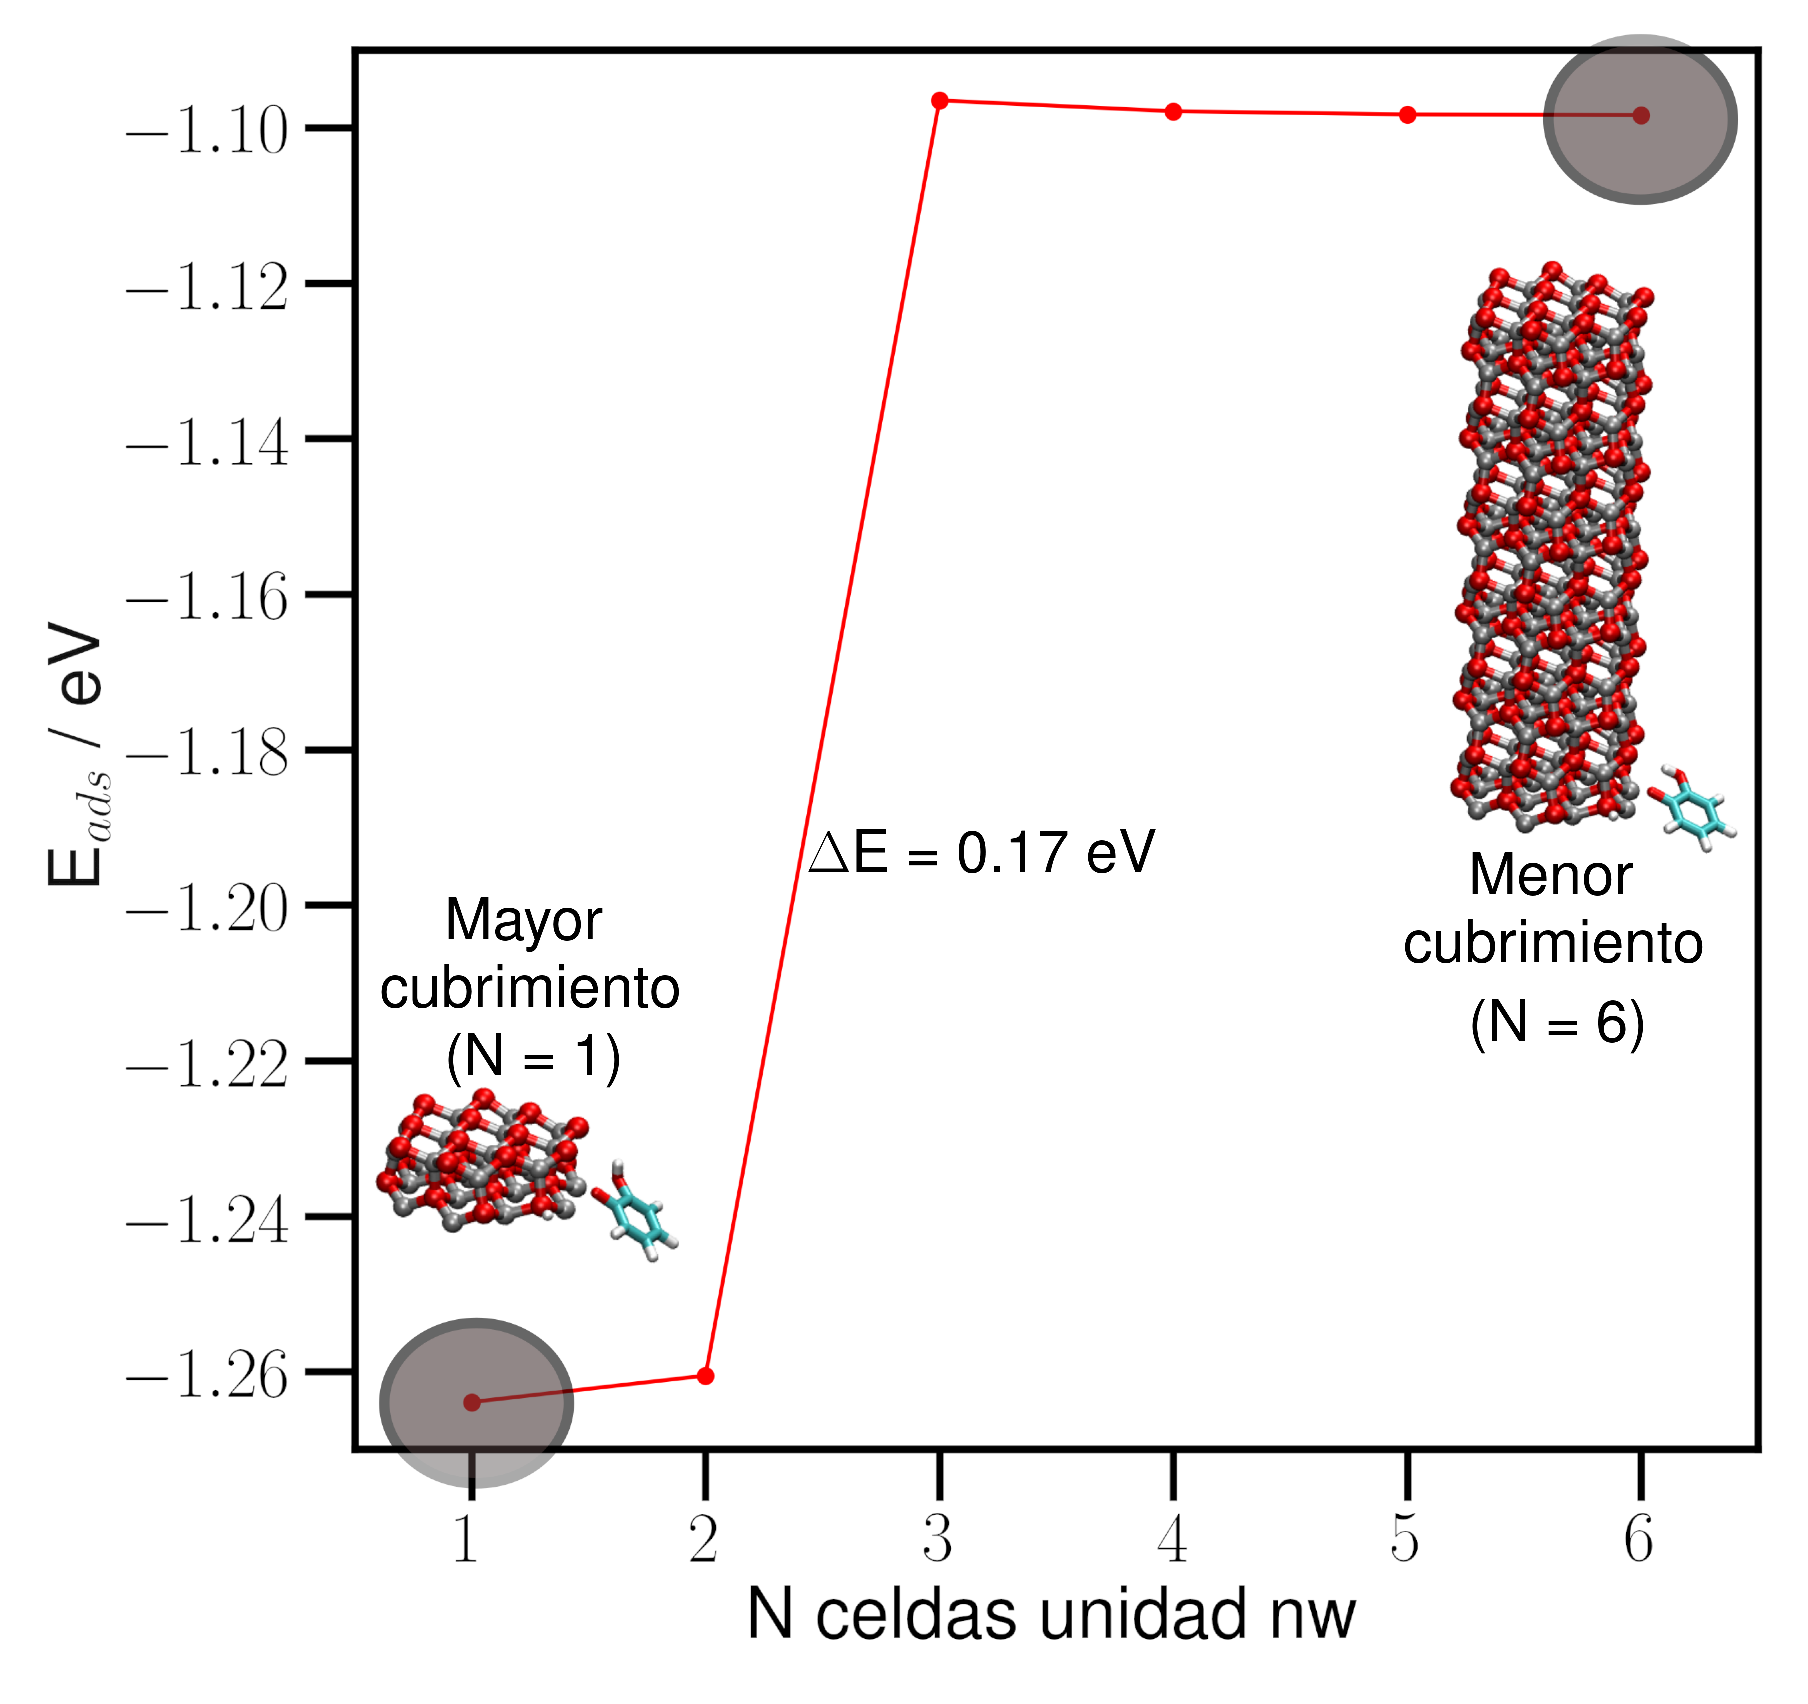
\includegraphics[height=11cm]{cap5/fig/e_ad_F.eps}
\caption{Energía de adsorción para los 6 sistemas estudiados en función de los distintos largos de superceldas de nw en relación a la celda unidad.}
\label{ead}
\end{figure}


La E$_{ad}$ se obtuvo de acuerdo a la siguiente ecuación:

\begin{equation}
 E_{ad} = E_{T(nw + CAT)} - E_{T(nw)} - E_{T(CAT)}
\end{equation}

donde E$_{T(nw + CAT)}$) es la energía total del complejo nw + CAT, E$_{T(nw)}$ la energía total del nw de ZnO y E$_{T(CAT)}$ de la molécula CAT. 


La figura \ref{ead} es un gráfico de E$_{ad}$ en función de N celdas unidad de nw, es decir, la cantidad de celdas unidad apiladas en el eje z: C$_1$ se correponde con N=1 y C$_2$ con N=2, etc. Se observan valores negativos de E$_{ad}$ entre $-1.1$ eV y $-1.3$ eV aproximadamente, reflejando una unión fuerte entre el adsorbato (CAT) y el adsorbente (nw). Estos resultados indican una quimisorción ya que las moléculas adsorbidas reaccionan químicamente con la superficie generando la formación de un enlace entre el CAT y el nw. A su vez, N=1 y N=2 (C$_1$ y C$_2$, respectivamente) muestran una E$_{ad}$ relativamente mayor (en valor absoluto) con respecto a los otros sistemas, la cual denota una estabilidad adicional en estos complejos que no se observa en otros. La diferencia de energía entre N=2 y N=3 es de $0.17$ eV y en principio se puede atribuír a distancias cortas entre catecoles. Las fuerzas de Van der Waals entre moléculas sólo justifican el complejo C$_1$ ya que en C$_2$ los CAT se encuentran a distancias lo suficientemente largas como para que esta interacción no tenga efecto. La causa por la cuál ocurre esta estabilización es la estudiaremos a lo largo del capítulo.

%A su vez, N=1 y N=2 (C$_1$ y C$_2$) muestran una E$_{ad}$ mayor en valor absoluto con respecto a los otros sistemas y se observa un delta de energía de $0.17$ eV entre N=2 y N=3 que corresponde a valores entre $13 - 15\%$ de la E$_{ad}$. Entonces, el hecho de que en C$_1$ y C$_2$ los catecoles se encuentren a distancias menores con respecto a los demás sistemas, otorga a los mismos una estabilidad adicional que no se observa en otros casos. 


%Esta estabilización puede deberse a {\bf (a)} interacciones tipo Van der Waals entre catecoles, {\bf (b)} diferencias conformacionales, {\bf (c)} interacciones entre los OM. La hipótesis {\bf (a)} sólo justificaría el complejo C$_1$ ya que en C$_2$ los catecoles se escuentran a distancias largas para considerar este tipo de interacciones. La hipótesis {\bf (b)} se pondrá a prueba a lo largo del capítulo. 

\subsection{Estructura de bandas}

El método de TB o combinación lineal de orbitales atómicos ({\bf CLOA}) es un método semiempírico que se utiliza principalmente para calcular la estructura de bandas y los estados de Bloch de una sola partícula de un material. El método de TB semi-empírico es simple y computacionalmente muy rápido y por lo tanto, tiende a usarse en cálculos de sistemas muy grandes, con más de unos pocos miles de átomos en la celda unidad.
 

\subsubsection{Cálculo de estructura de bandas dentro del formalismo TB}

%Para sistemas que contienen hasta unos cientos o miles de átomos, podemos utilizar la DFT para encontrar la densidad del estado fundamental real y la energía del estado fundamental del sistema que interactúa sin calcular explícitamente la función de onda de muchos electrones. En un cálculo de este tipo obtenemos energías aproximadas de una sola partícula que, en la práctica, a menudo dan una aproximación razonable a la estructura de bandas real del cristal. En sistemas aún más grandes, con alrededor de $10.000$ o más átomos, ya no podemos usar cálculos de DFT autoconsistentes para tener en cuenta la interacción completa. 

Cuando se calcula la estructura de bandas y un conjunto de estados de una sola partícula aproximados utlizando el método de TB, se intenta incluir los efectos de la interacción de una manera semiempírica, utilizando parámetros que podemos ajustar y que coincidan con el experimento. El punto de partida de todos los enfoques semiempíricos es la física. En los metales, por ejemplo, los electrones son casi libres, por lo que podemos tratar los estados de una sola partícula en términos de ondas planas. También podemos adoptar un enfoque diferente y asumir que los estados en un cristal son combinaciones de funciones de onda de átomos aislados, lo cual es más probable que sea el caso de los aislantes o semiconductores. A continuación, resolveremos la ecuación de Schr\" odinger de una sola partícula para los estados en un cristal expandiendo los estados de Bloch en términos de una combinación lineal de orbitales atómicos \cite{Roy2015}. 

En un cristal, definimos el hamiltoniano de una sola partícula como  

\begin{equation}
 H = H_{at} + \Delta U,
\end{equation}


donde $H_{at}$ es el hamiltoniano de un solo átomo y $\Delta U$ comprende todas las diferencias entre el verdadero potencial en el cristal y el potencial de un átomo aislado. Suponemos $\Delta U \rightarrow 0$ en el centro de cada átomo del cristal. Los estados de una sola partícula en el cristal son entonces $\Psi_{n {\bf k}}({\bf r})$, donde 

\begin{equation}
H \, \Psi_{n {\bf k}}({\bf r}) = E_{n {\bf k}}  \Psi_{n {\bf k}}({\bf r}),
\end{equation}

el índice de banda está etiquetado por n, y {\bf k} es un vector de onda de la primera zona de Brillouin. Las {\bf funciones de onda atómicas}, $\phi_{i}({\bf r})$, son estados propios de $H_{at}$,

\begin{equation}
H_{at} \, \phi_{i}({\bf r}) = \epsilon_{i}  \phi_{i}({\bf r}),
\end{equation}

donde $\epsilon_{i}$ es la energía del nivel de energía i en un átomo aislado. Estas funciones de onda decaen rápidamente alejándose de $r = 0$ y, por lo tanto, la integral de solapamiento, $\gamma (|{\bf R}|) = \int \phi^* ({\bf r})\, H\, \phi ({\bf r} + {\bf R})  \, d{\bf r}$, es pequeña entre funciones de onda ubicadas en sitios atómicos separados (${\bf R} \neq 0$) en el cristal (ver figura \ref{tb_orb}). 

%\begin{equation}
%\int{\phi_{i}^*({\bf r})\phi_{j}({\bf r} + {\bf R} ) \, d{\bf r}} = \left\lbrace
%\begin{array}{ll}
%1 & \textup{si} \hspace{0.2cm} i=j \hspace{0.2cm} y \hspace{0.2cm} {\bf R} = 0  \\
%0 & \textup{de otra manera}
%\end{array}
%\right.
%\label{eq:solapamiento}
%\end{equation}

\vspace{1cm}

\begin{figure}[!htb]
\centering
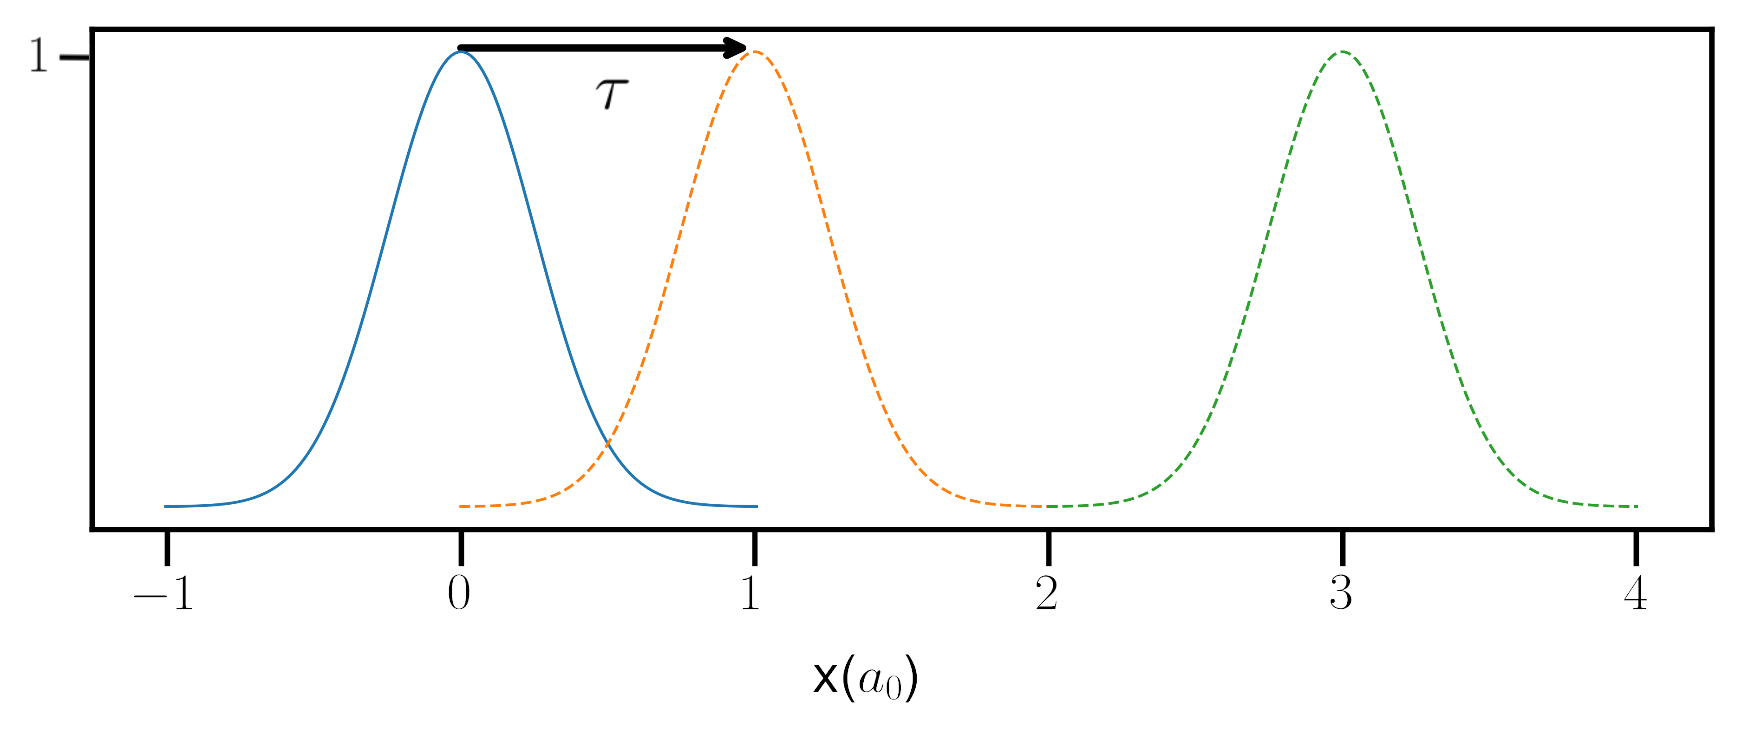
\includegraphics[height=6cm]{cap5/fig/gauss_final.eps}
\caption{Esquema de los orbitales atómicos en un cristal 1D con átomos separados por $a_0$. Los vectores de traslación son ${\bf R} = 0$,$\pm a_0{\bf i}$, $\pm 2a_0{\bf i}$, $\pm 3a_0{\bf i}$,$...$, donde ${\bf i}$ es un vector unitario en la dirección $x$. Se muestra en el diagrama uno de los vectores vecinos más cercanos, $\tau = a_0{\bf i}$ y las líneas de puntos verticales denotan los bordes de la celda unidad que contiene un solo átomo. El gráfico azul muestra un orbital atómico centrado en un átomo en $r=0$, mientras que los gráficos con líneas discontinuas muestran orbitales centrados en $r+\tau$ y $r+3\tau$. Aquí asumimos que la integral de superposición,$\int \phi^* ({\bf r})\, H\, \phi ({\bf r} + {\bf R})  \, d{\bf r}$, es sólo significativa cuando $|{\bf R}|$ está cerca de $|\tau|$.}
\label{tb_orb}
\end{figure}


\newpage

Los estados de una sola partícula, $\Psi_{n {\bf k}}({\bf r})$, deben obedecer el {\bf teorema de Bloch}, 

\begin{equation}
\displaystyle \Psi_{n {\bf k}}({\bf r} + {\bf R}) =  e^{i {\bf k}.{\bf R}} \Psi_{n {\bf k}}({\bf r}), 
\end{equation}

donde ${\bf R}$ es un vector de traslación espacial real del cristal. Un solo orbital atómico no satisface el teorema de Bloch, pero podemos plantear fácilmente una CLOA que sí lo haga,  

\begin{equation}
\displaystyle \Psi_{n {\bf k}}({\bf r}) = \frac{1}{\sqrt{N}} \sum_{{\bf R}} e^{i {\bf k}.{\bf R}} \phi_n ({\bf r}-{\bf R}), 
\end{equation}

donde hay N sitios de red en el cristal y el factor $\frac{1}{\sqrt{N}}$ asegura que el estado de Bloch esté normalizado. 

\begin{itemize}
 \item Banda s en un cristal 1D
\end{itemize}

Imaginemos un cristal con vectores de traslación {\bf R}, que tiene un átomo en la celda unidad, y donde solo los orbitales atómicos s $\phi_{s}({\bf r})$ contribuyen a los estados del cristal. En el caso de un {\bf cristal 1D}, los vectores de traslación son ${\bf R} = na_0{\bf i}$ donde n es un número entero, $a_0$ es la separación atómica e {\bf i} es un vector unitario en la dirección x. En este caso, hay dos vectores de traslación vecinos más cercanos $\tau = \pm a_0 {\bf i}$. Entonces solo hay 1 banda (n = 1) y solo hay un estado de Bloch que podemos construir,

\begin{equation}
\displaystyle \Psi_{{\bf k}}({\bf r}) = \frac{1}{\sqrt{N}} \sum_{{\bf R}} e^{i {\bf k}.{\bf R}} \phi_s ({\bf r}-{\bf R}), 
\label{eq:psi_single_s_band}
\end{equation}

En este caso simple podemos encontrar la {\bf relación de dispersión} (la relación entre la energía y el vector de onda) simplemente calculando el valor esperado o de expectación de la energía, 

\begin{align}
E({\bf k}) &= \int \Psi^*_{{\bf k}} ({\bf r})\, H\, \Psi_{\bf k} ({\bf r})  \, d{\bf r} \label{exp_e_paso1} \\
& = \frac{1}{\sqrt{N}} \sum_{{\bf R}} \sum_{{\bf R'}} e^{i {\bf k}.({\bf R'} -{\bf R}) } \int \phi^*_s ({\bf r} - {\bf R})\, H\, \phi_s ({\bf r} - {\bf R'})  \, d{\bf r} \label{exp_e_paso2} \\ 
&= \frac{1}{\sqrt{N}} \sum_{{\bf R}} \sum_{{\bf R'}} e^{i {\bf k}.({\bf R'} - {\bf R}) } \int \phi^*_s (x)\, H\, \phi_s (x - ({\bf R} - {\bf R'}))  \, d{\bf x} \label{exp_e_paso3}\\
&= \sum_{{\bf R''}} e^{i {\bf k}.{\bf R''}} \int \phi^*_s (x)\, H\, \phi_s (x - ({\bf R} - {\bf R'}))  \, d{\bf x} \label{exp_e_paso4}\\
&= \epsilon_s + \sum_{\tau} e^{i {\bf k}.\tau} \, \gamma(|\tau|) \label{exp_e_paso5}
\end{align}

donde las integrales están sobre todo el espacio. La expresión final (ec. \ref{exp_e_paso5}) para el valor de expectación se obtuvo a partir de la ec. \ref{exp_e_paso1} siguiendo los siguientes pasos:

\begin{enumerate}
 \item Sustitución de $\Psi_{{\bf k}}({\bf r})$ de la ec. \ref{eq:psi_single_s_band} en la ec. \ref{exp_e_paso1} 
 \item Cambio de variables de {\bf r} a x = {\bf r} - {\bf R} en la ec. \ref{exp_e_paso3} 
 \item Reemplazo de {\bf R'}-{\bf R} con el vector de traslación {\bf R''} = {\bf R'}-{\bf R} en la ec. \ref{exp_e_paso4} debido a que la suma sobre {\bf R'} tiene en cuenta todos los vectores de traslación, obtendremos el mismo resultado al sumar sobre otro vector de traslación. Una vez que hacemos esto, reconocemos que la suma de {\bf R} simplemente da un factor de N, un término para cada uno de los N valores posibles de R. 
 \item Ahora en la ec. \ref{exp_e_paso5} podemos separar diferentes términos en la suma de {\bf R''} considerando el rango de los orbitales s atómicos. En el primer término, es decir {\bf R''=0}, se observa la energía del orbital atómico $\phi_s$ en un átomo aislado, $\epsilon_s$ y para el segundo término la sumatoria sobre {\bf R''} pequeño como por ejemplo {\bf R''} = $\tau$ que es el vector de traslación entre un átomo y sus vecinos más cercanos y por último se reemplazó la integral de solapamiento, $\gamma$, con un parámetro cuyo valor coincida con el experimento.
 \end{enumerate}
  
 En un cristal 1D sabemos que $\tau = \pm a_0 {\bf i}$ y que los únicos vectores de onda significativos, {\bf k}, también deben estar en la dirección de {\bf i}, de modo que {\bf k} = k{\bf i}. Entonces, 

 \begin{align}
E({\bf k}) &= \displaystyle \epsilon_s + \gamma(a_0) (e^{ika_0} + e^{-ika_0}) \nonumber \\
           &= \epsilon_s + 2\gamma(a_0) \cos(k a_0) \label{exp_e_final}
\end{align}

La ec. \ref{exp_e_final} es la relación de dispersión para una sola banda s en un cristal 1D. Describe cómo varía la energía con el momento del cristal,{\bf ancho de banda}, y también nos dice el {\bf ancho de banda}. 

En general, un material tendrá más de un átomo en la celda unidad y las bandas tendrán contribuciones de más de un tipo de orbital. En un cristal con N$_b$ bases atómicas (y donde solo un tipo de orbital atómico contribuye a los estados de banda) podemos hacer Nb combinaciones lineales de orbitales atómicos que satisfagan el teorema de Bloch, los índices i = 1, 2,. . . ,N$_b$ etiquetan cada uno de los diferentes átomos de la base y los ${\bf R'}_i$ son vectores de traslación entre átomos de tipo $i$. Sin embargo, es muy fácil generalizar este formalismo para tratar con múltiples tipos de orbitales, todo lo que tenemos que hacer es usar el índice i para etiquetar diferentes sitios base y diferentes tipos de orbitales.

Los SC son sólidos donde los átomos constituyen una red tridimensional infinita. El solapamiento de los orbitales atómicos va más allá de los primeros vecinos, extendiéndose por toda la red; resulta entonces una configuración de estados deslocalizados muy próximos entre sí, que forman bandas de estados electrónicos permitidos. Entre las bandas, hay intervalos de energía en los cuales no hay estados electrónicos permitidos (GAP) mientras que las bandas de valencia y conducción surgen del solapamiento de los niveles atómicos de los electrones de valencia. La figura \ref{origen_bandas} es un esquema que ilustra el origen de las bandas dentro del formalismo TB. En un átomo aislado tenemos un conjunto de niveles atómicos individuales, por ejemplo, 1s, 2s, 2p, etc. En un cristal con N átomos y superposición cero entre estados atómicos tendríamos N niveles degenerados para cada estado atómico. A medida que aumenta la integral de solapamiento, estos niveles se amplían en bandas, cada una de las cuales contiene N valores diferentes de {\bf k} permitidos. 

\begin{figure}[!htb]
\centering
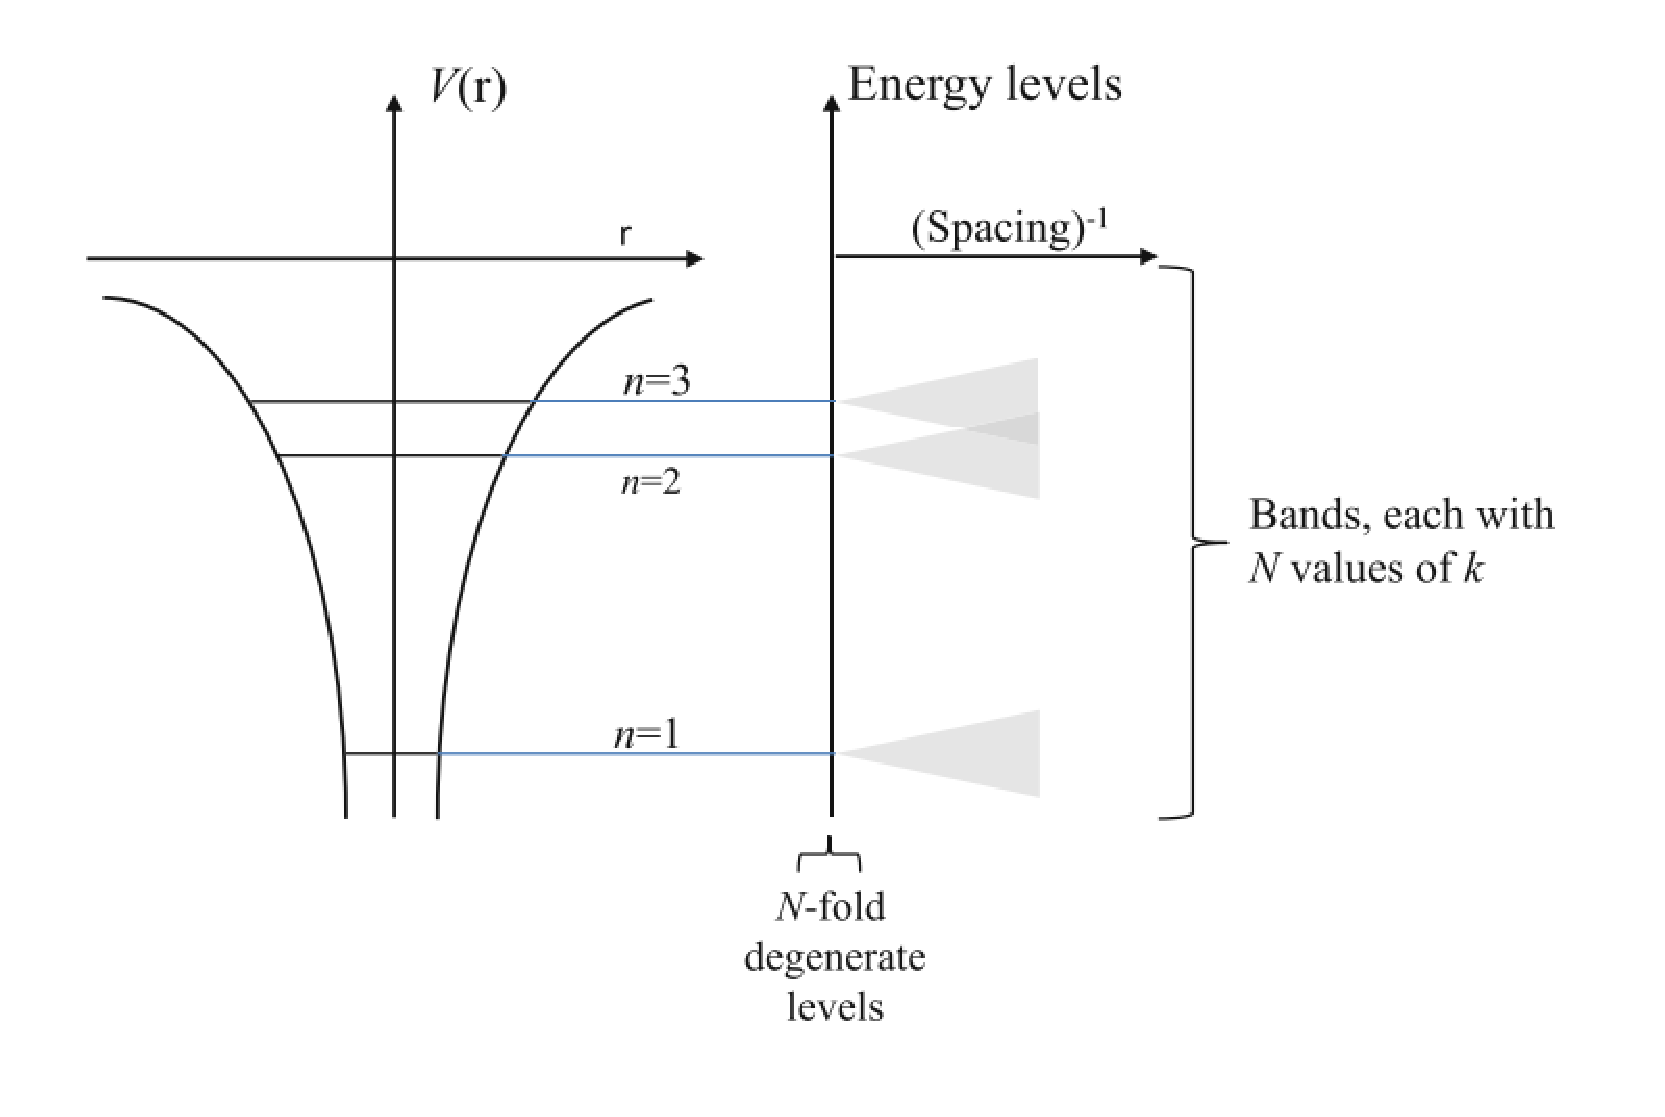
\includegraphics[height=6cm]{cap5/fig/formacion_bandas.eps}
\caption{ {\bf (Izquierda)} los niveles electrónicos no generados en un solo átomo. {\bf (Derecha)} niveles de energía para los átomos de N en un cristal, representados como una función de la integral de solapamiento o la inversa del espacio atómico. Extraído de \cite{Dresselhaus2018}}
\label{origen_bandas}
\end{figure}


\subsubsection{Cálculo de estructura de bandas en sistemas CAT-nw}

La estructura electrónica de bandas de un SC dado es fundamental para determinar su potencial utilidad. En consecuencia, un conocimiento preciso de la estructura de bandas es fundamental para desarrollar dispositivos eficientes. Dicho esto, primero calculamos con dftb+ las bandas para el SC aislado, es decir, para las 6 superceldas de ZnO wurtzita de distinta altura tal como muestra la figura \ref{bandas_nw_aislados}. En la misma se muestran los gráficos de energía en función del vector de onda {\bf k}, en particular los puntos críticos de alta simetría G y Z de la zona de brillouin (ZB) donde G es el origen. 

\begin{figure}[!htb]
\centering
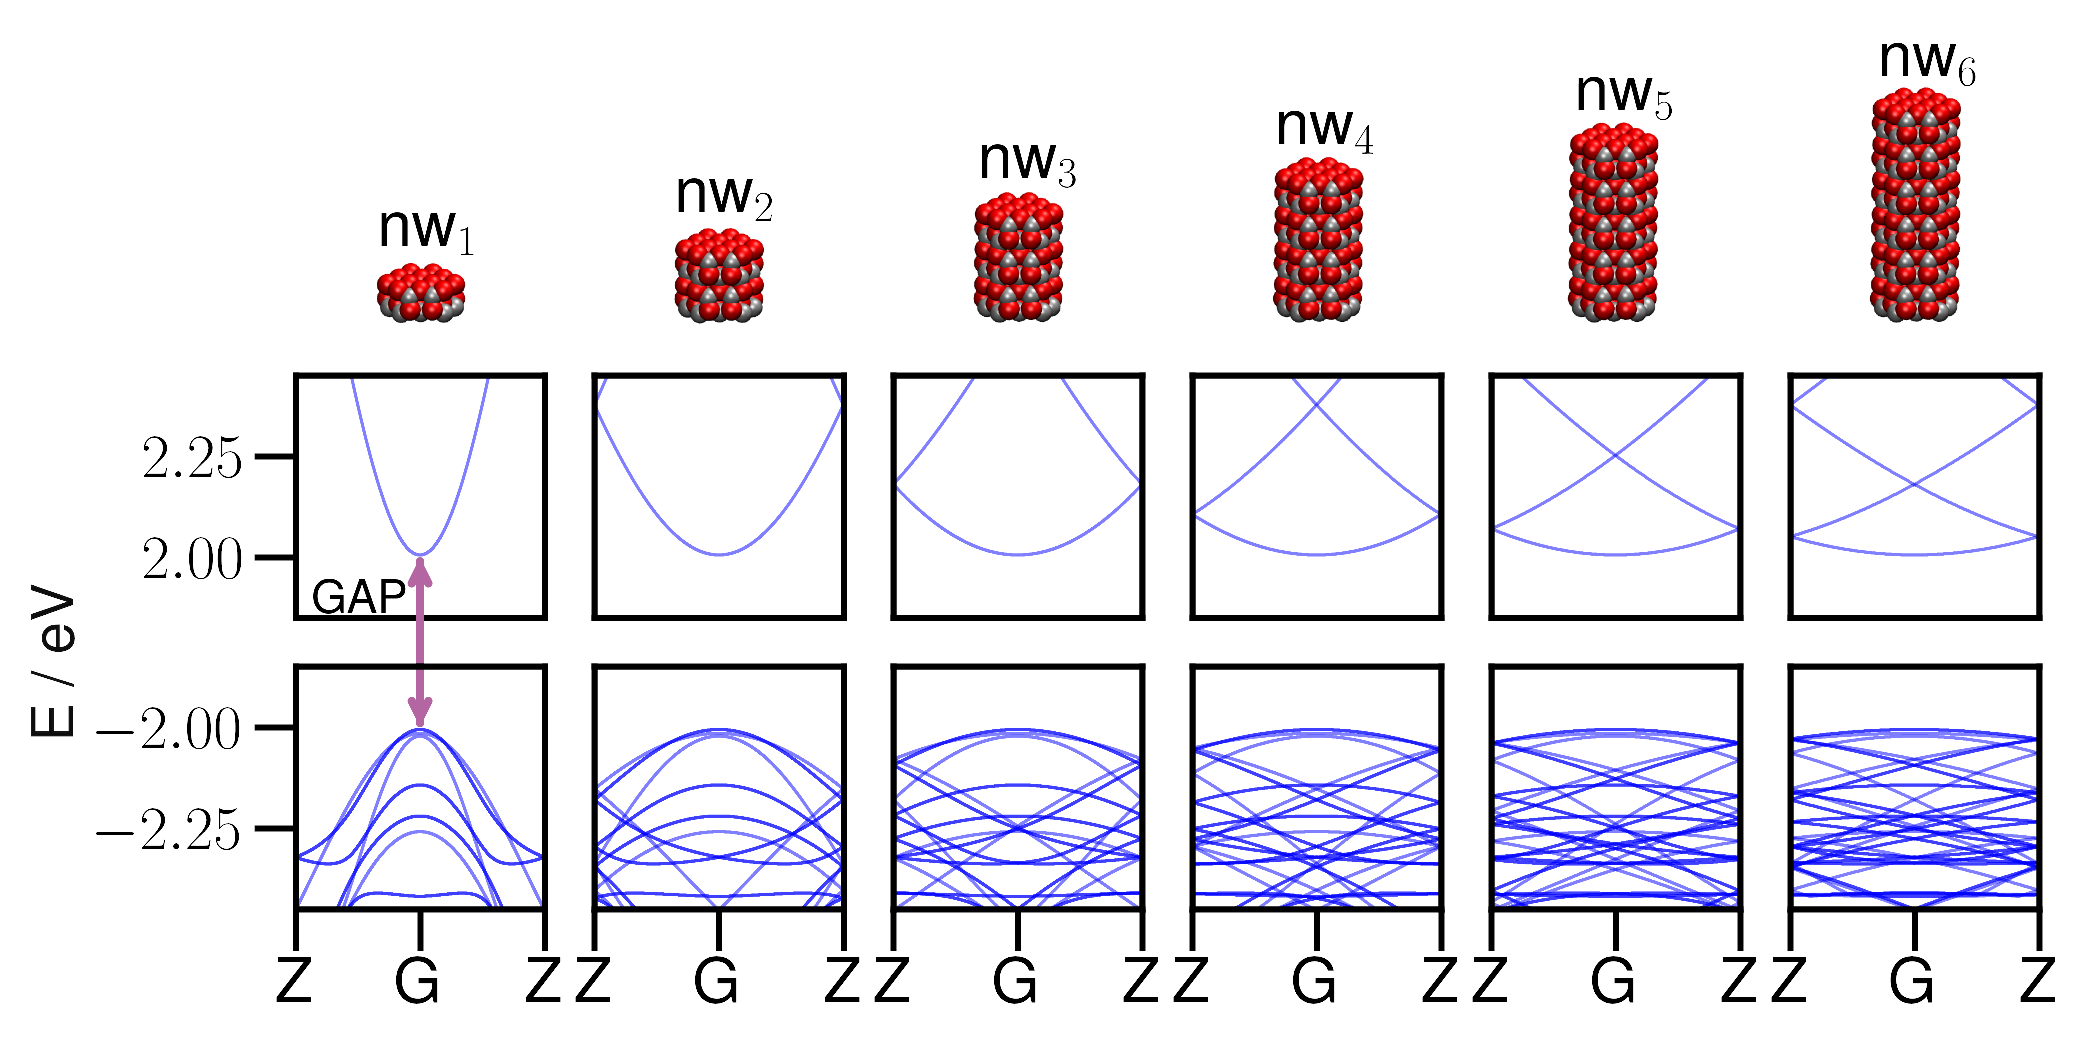
\includegraphics[height=7cm]{cap5/fig/bandas_nw_F.eps}
\caption{Estructura de bandas simuladas con dftb+ de los nws aislados. Se grafica la energía en función del vector de onda {\bf k}}
\label{bandas_nw_aislados}
\end{figure}


En los gráficos de bandas se pueden observar las bandas de valencia y conducción, la BV con valores negativos de energía desde $-2$ eV y la BC con energías positivas a partir de $2$ eV. El GAP es de aproximadamente $4.00$ eV como muestra la flecha, calculado como la diferencia de energía entre el borde de la BC y el borde de la BV que se encuentra en G (mínima energía). Este valor se mantiene constante a medida que aumenta la altura en las superceldas, la cual tiene sentido ya que estamos tratando con el mismo material independientemente de la cantidad de átomos utilizados. 

Si bien el GAP se mantiene constante, se pueden observar cambios en las bandas como por ejemplo el plegamiento de las mismas a medida que aumenta la altura o el número de átomos en la supercelda. Este efecto es típico en sistemas periódicos y se puede explicar utilizando un sistema simple como por ejemplo una cadena de moléculas 1D o un polímero, con 1 o 2 átomos por celda unidad tal como lo describe Yang \emph{et al.} en su trabajo publicado en 2018 \cite{Yang2018} (ver figura \ref{plegado}).

\begin{figure}[!htb]
\centering
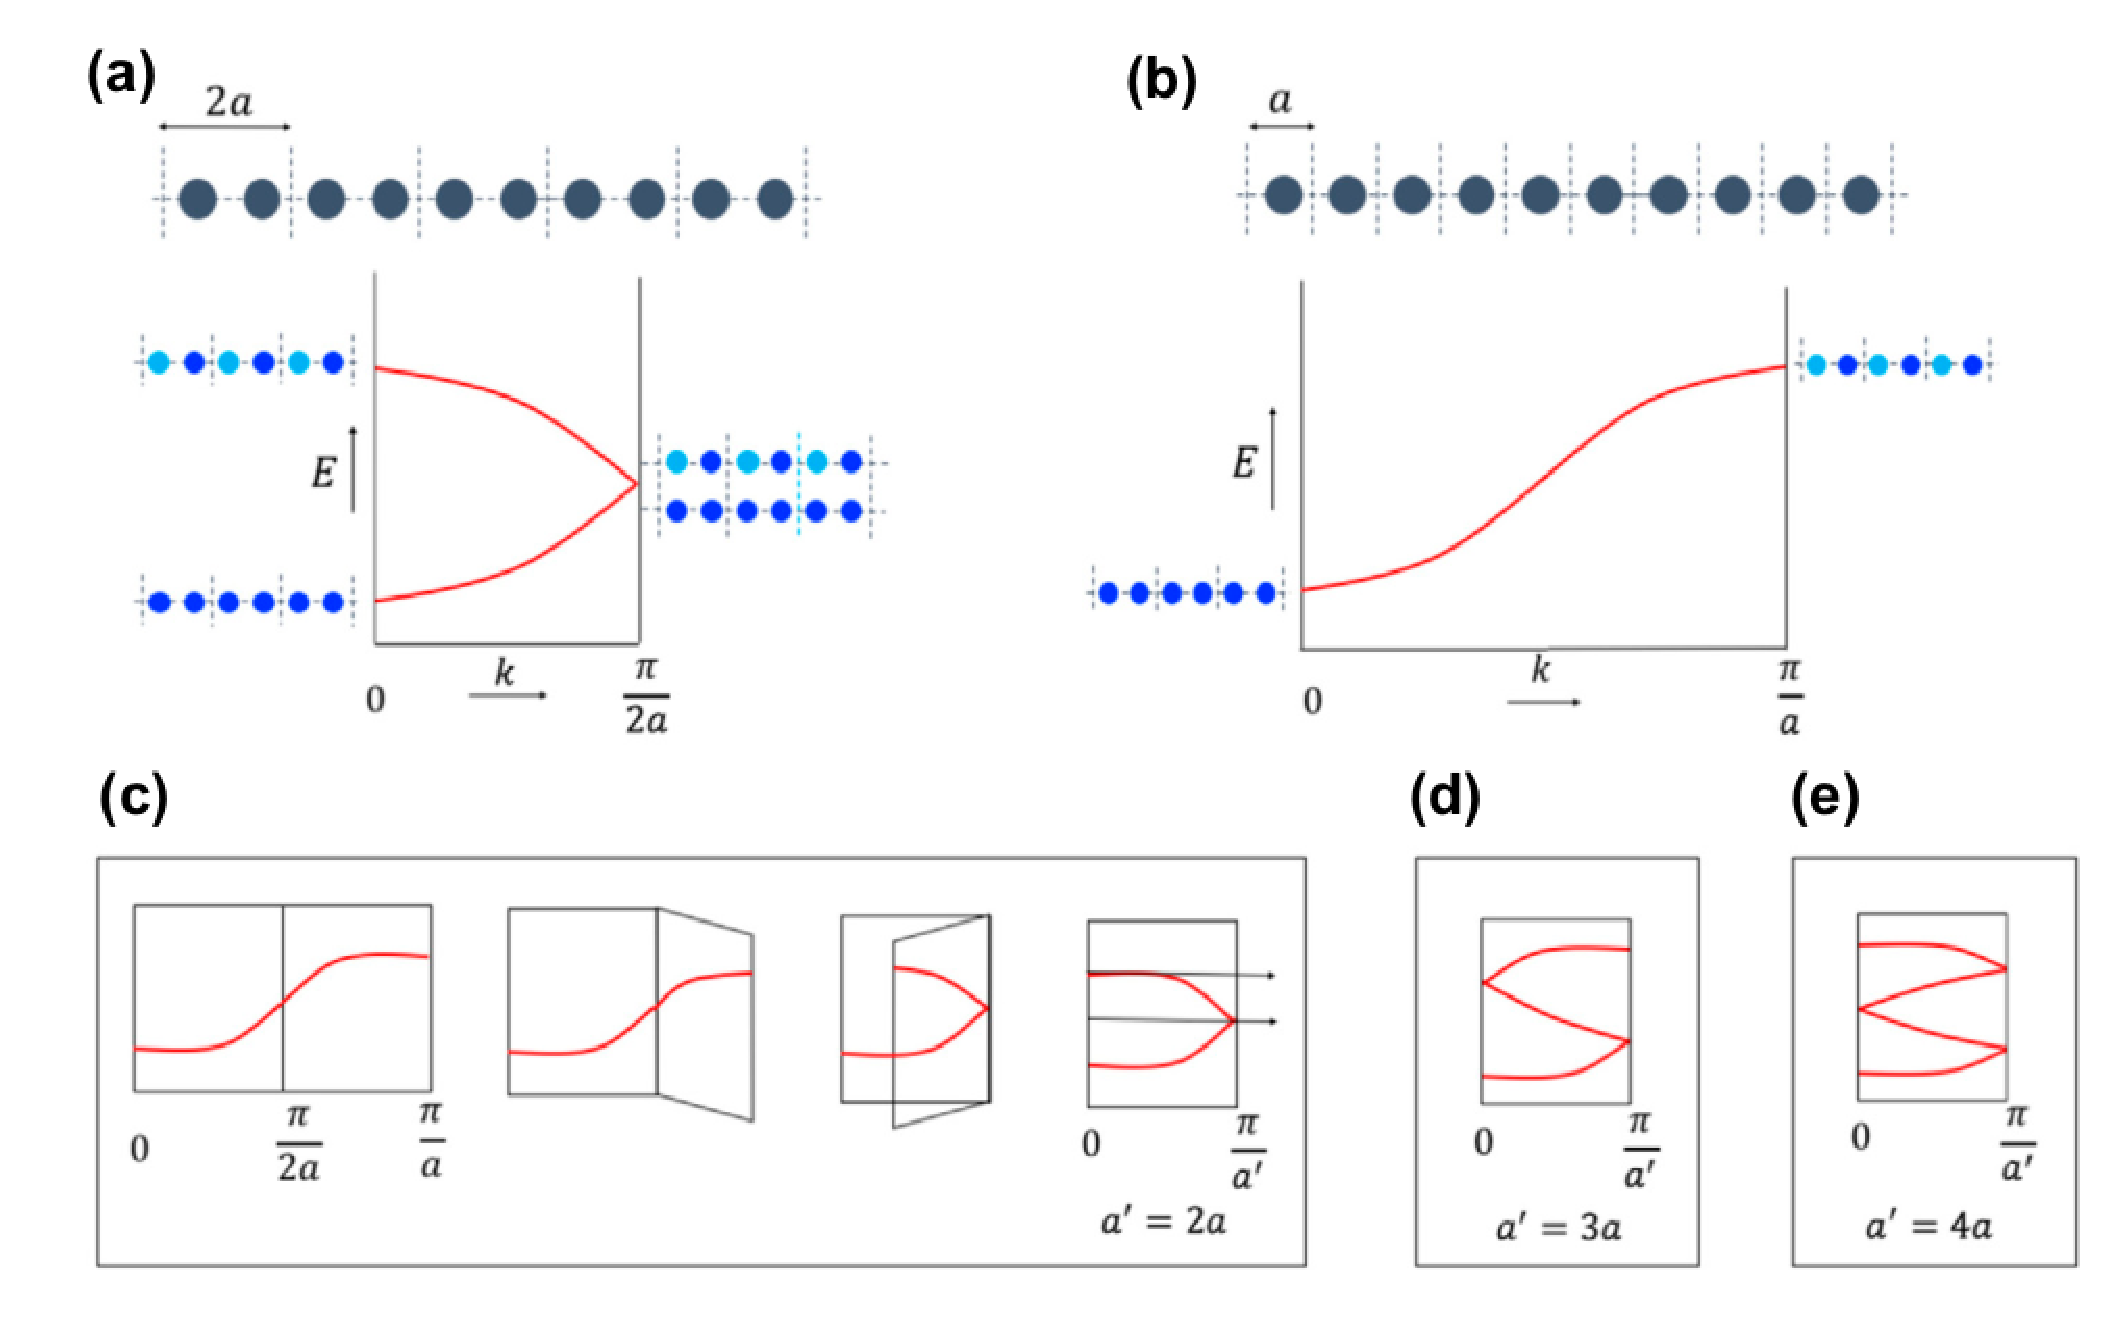
\includegraphics[height=7cm]{cap5/fig/plegado.eps}
\caption{Plegado de bandas en polímeros unidimensionales. {\bf(a)} Estructura de bandas de un polímero en el que hay dos átomos por celda unidad. Las bandas contienen dos ramas que se cruzan en ${\bf k}= \pi/2a$. {\bf(b)} Estructura de banda de un polímero en el que hay un átomo por celda unidad. La zona de brillouin se duplica porque la celda unidad es la mitad que en {\bf(a)}. {\bf(c)} Producción de la estructura de la banda en {\bf(a)} mediante el plegado de la estructura de la banda en {\bf(b)}. {\bf(d)} - {\bf(e)} La ampliación de la celda unidad provoca la multiplicidad de bandas. Las bandas se doblan tres veces cuando la celda unidad se triplica, cuatro veces cuando se cuadriplica. Extraído de \cite{Yang2018}}
\label{plegado}
\end{figure}


Si consideramos en primer lugar el sistema con 2 átomos por celda unidad como se expone en la figura \ref{plegado}{\bf(a)}, observamos que las bandas contienen 2 ramas, una hacia arriba desde los orbitales enlazantes y una hacia abajo desde los orbitales antienlazantes. Las mismas se cruzan en ${\bf k}= \pi/2a$ donde $2a$ es la longitud de la celda. Cuando la celda tiene 1 sólo átomo como se muestra en {\bf(b)}, la ZB se duplica ${\bf k}= \pi/a$ debido a que la longitud de la celda unidad es la mitad con respecto al caso anterior. Dado que la estructura de bandas no debería depender de la elección de la celda unidad, la estructura de bandas de {\bf(a)} y {\bf(b)} tienen que brindar la misma información. Esto podría entenderse como que la figura {\bf(a)} es la figura {\bf(b)} “plegada”, tal como se muestra en {\bf(c)}. Por último, las figuras {\bf(d)} y {\bf(e)} muestran que el proceso de plegado de bandas se puede continuar, es decir que si la celda unidad se triplica, la banda se doblará como se observa en {\bf(d)} y así sucesivamente. 


\begin{figure}[!htb]
\centering
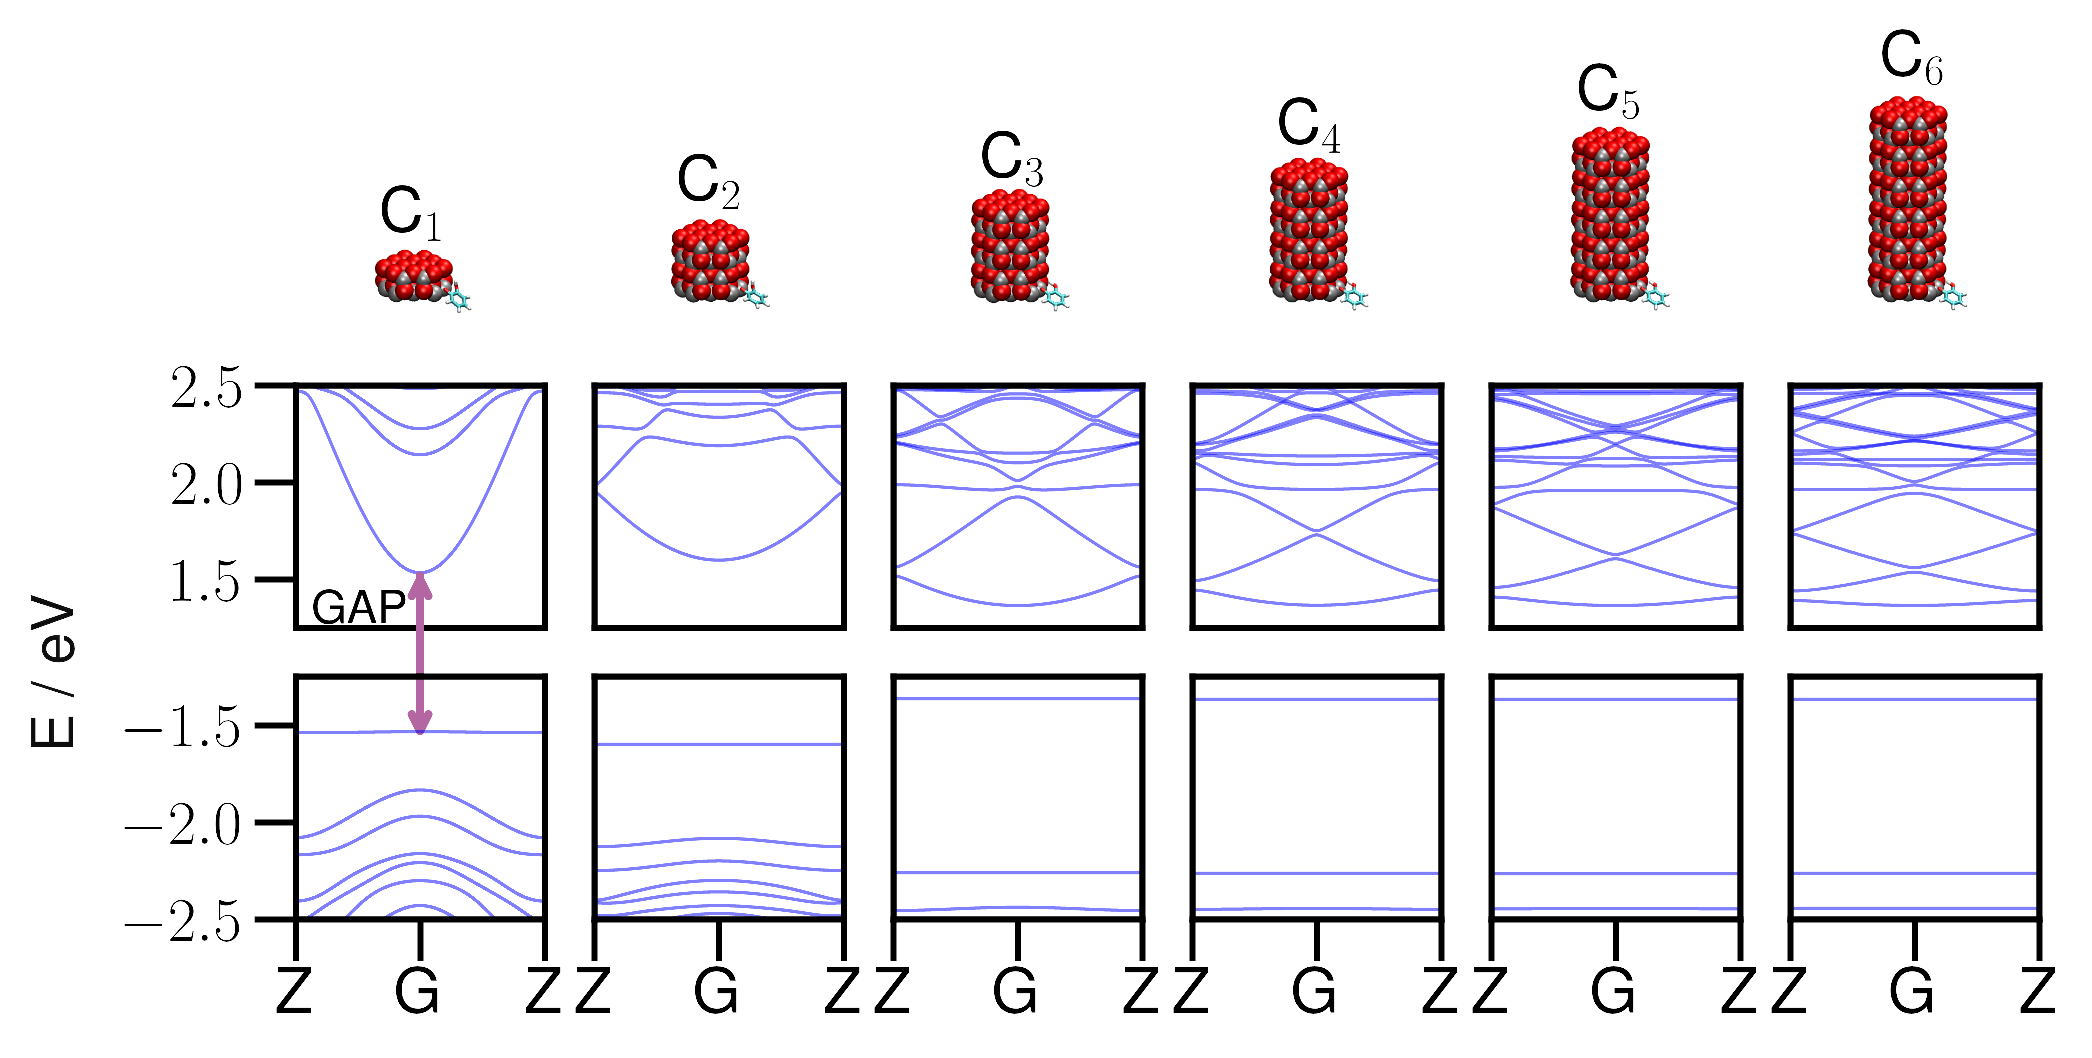
\includegraphics[height=7cm]{cap5/fig/bandas_C_F.eps}
\caption{Estructura de bandas simuladas con dftb+ de los nws aislados. Se grafica la energía en función del vector de onda {\bf k}}
\label{bandas_complex}
\end{figure}


A continuación en la figura \ref{bandas_complex} se muestran los gráficos de los cálculos de estructura de bandas para los complejos CAT-nw, es decir después de que el catecol se adsorba a la superficie del nw. A simple vista se observan varias diferencias con respecto a las bandas del nw aislado (ver figura \ref{comp_bandas}), sin embargo, es importante destacar que tanto el plegado de bandas se sigue observando en las bandas porque sigue siendo un sistema periódico. La disminución a aproximadamente $3$ eV del GAP es uno de los cambios más notables, este valor oscila en los sistemas más pequeños hasta estabilizarse con las superceldas de más átomos, es decir los complejos C$_3$, C$_4$ C$_5$ y C$_6$. 

\begin{figure}[!htb]
\centering
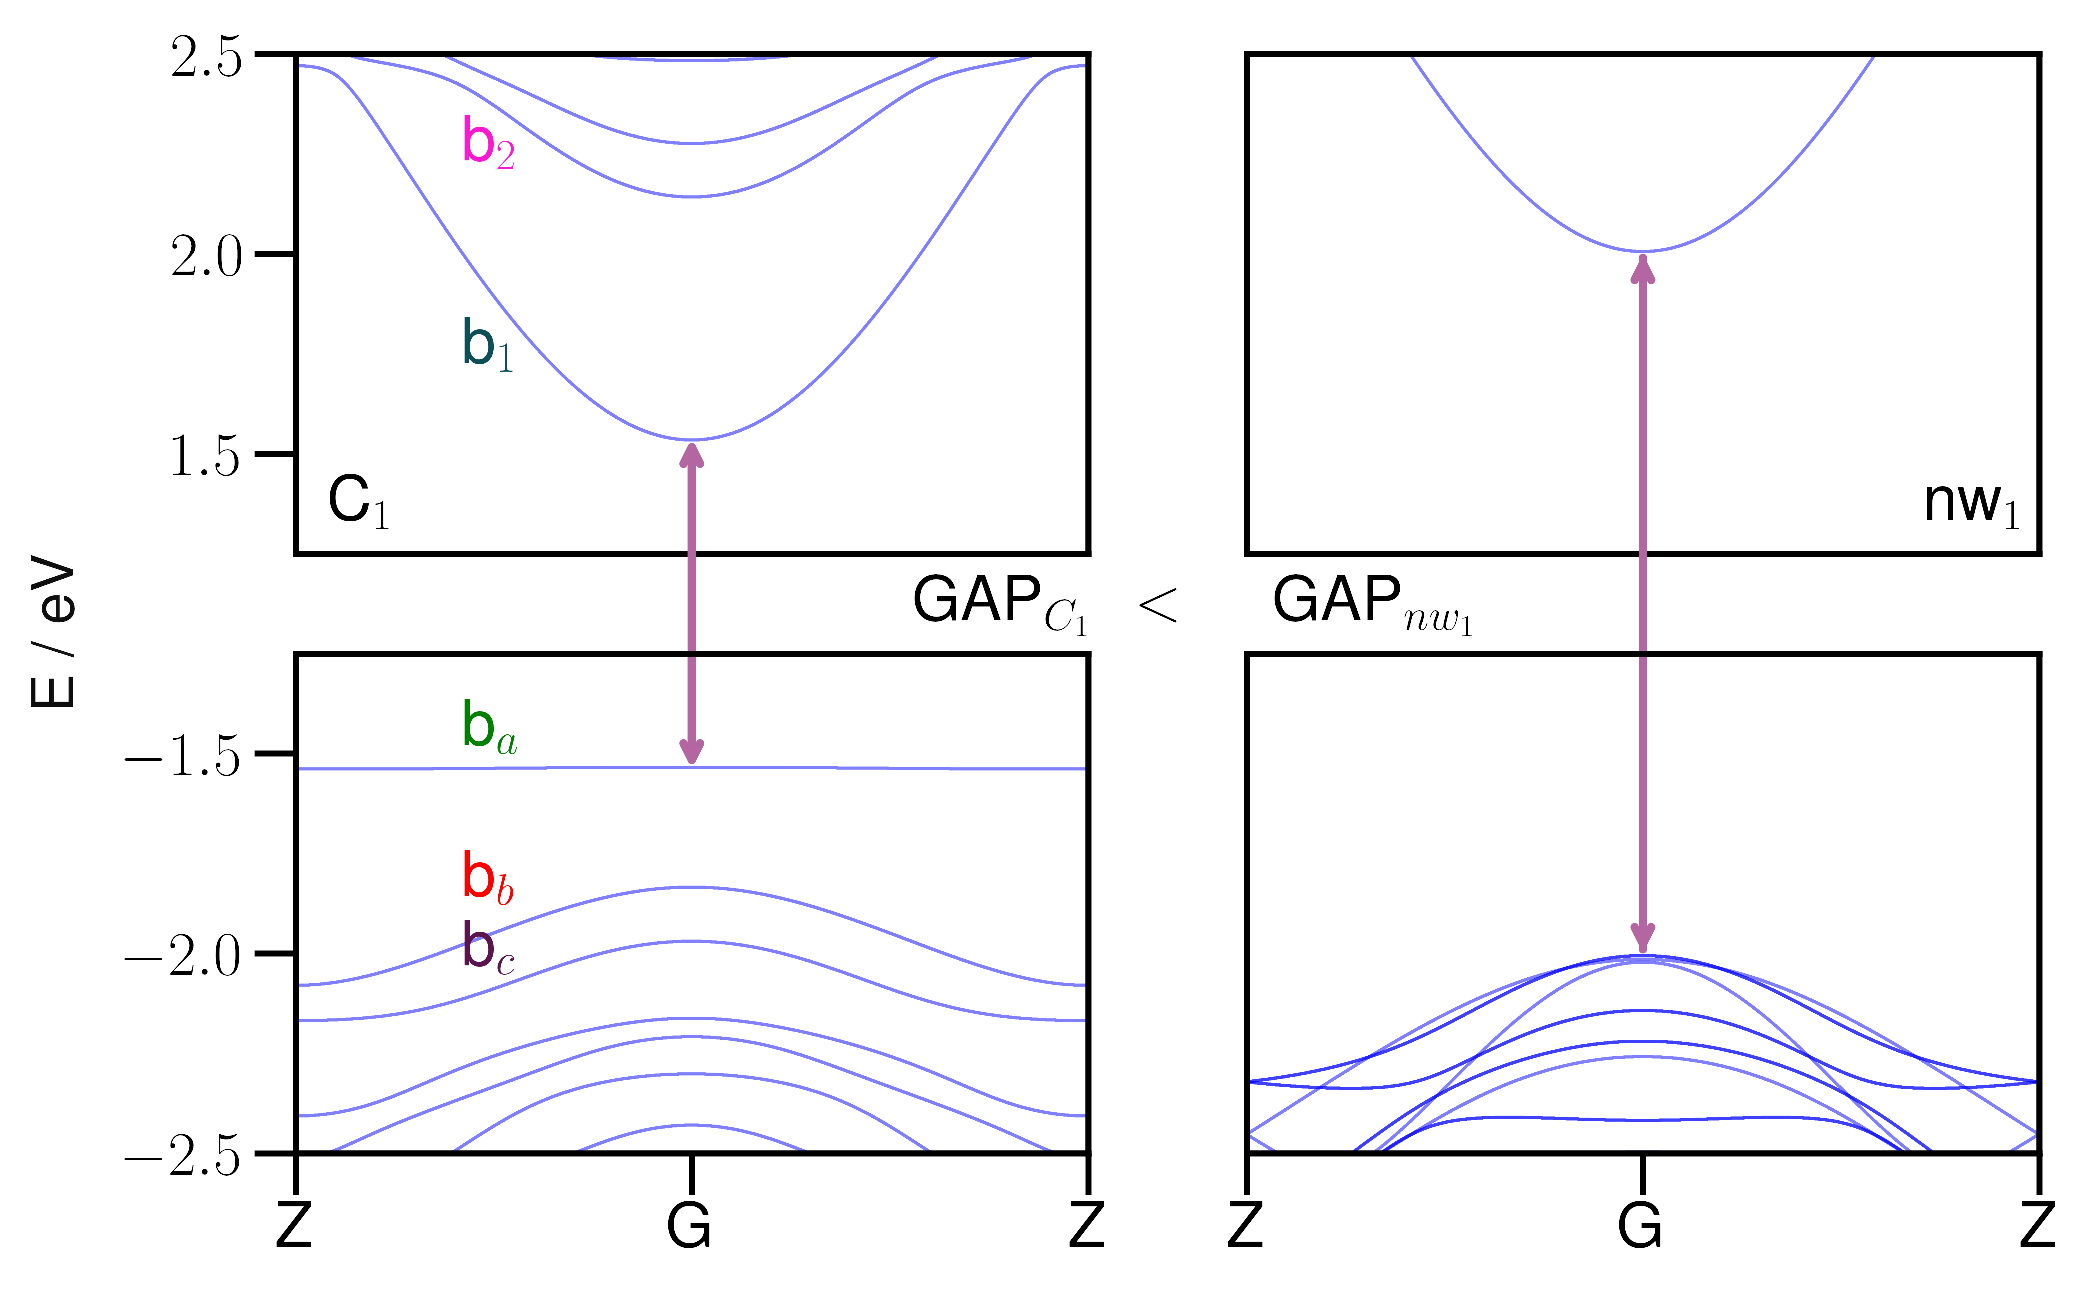
\includegraphics[height=7cm]{cap5/fig/comp_bandas.eps}
\caption{Comparación de los gráficos de estructura de bandas de C$_1$ {\bf (izquierda)} y nw$_1$ {\bf (derecha)}}
\label{comp_bandas}
\end{figure}

\newpage

También hay importantes diferencias en la BV y por esta razón nos enfocaremos (en este capítulo) en el análisis de las 3 bandas de mayor energía para cada sistema como muestra la figura \ref{comp_bandas}. Asignamos a la banda más energética de la BV como b$_a$ y las que siguen en energía como b$_b$ y b$_c$. Para estudiar cuáles son las contribuciones en cada una de las bandas recurrimos a las gráficas de orbitales moleculares (OM) (en el punto G) como se muestra a continuación en la figura \ref{om}. Realizando un análisis en simultáneo de la estructura de bandas y los OM podremos obtener una visión más clara de los cambios en la estructura electrónica al formarse el complejo.  

\begin{figure}[!htb]
\centering
\includegraphics[height=13.5cm]{cap5/fig/om.eps}
\caption{Esquema de los orbitales moleculares para cada uno de los sistemas estudiados correspondientes al punto G de la bandas b$_a$ (verde), b$_b$ (rojo) y b$_c$ (violeta) de la BV.}
\label{om}
\end{figure}


En este contexto, es importante destacar la aparición de una nueva banda, b$_a$, en la BV del gráfico de estructura de bandas de los complejos como consecuencia de la absorción del CAT, la cual cuenta con una energía alrededor de $-1.5$ eV y es una de las mayores responsables de la disminución del GAP. El orbital molecular correspondiente a esta banda se encuentra localizado en el colorante en todos los sistemas (ver figura \ref{om}), de manera que la misma está asociada al catecol. Las bandas que no dependen del vector de onda {\bf k} como ocurre en este caso, son llamadas bandas sin dispersión. 

Conforme a la figura \ref{bandas_complex}, b$_b$ y b$_c$ son bandas sin dispersión solo para los complejos C$_3$, C$_4$, C$_5$ y C$_6$. A priori podríamos decir que también están relacionadas con transiciones del catecol en acuerdo con los resultados obtenidos para b$_a$. En los sistemas C$_1$ y C$_2$, en cambio, las bandas b$_b$ y b$_c$ tienen dispersión ya que en estos casos la energía depende de {\bf k}. Si estudiamos los gráficos de la figura \ref{om} correspondientes a estas bandas (rojo para b$_b$ y violeta para b$_c$) encontramos 2 tipos de OM. El primer tipo corresponde a los complejos C$_3$, C$_4$, C$_5$ y C$_6$ donde los OM de la banda b$_b$ se encuentran localizados en el catecol y los OM de la banda b$_c$ están localizados en el sitio de unión CAT-nw, tal como lo habíamos predecido. Es decir que efectivamente las bandas sin dispersión involucran OM localizados con contribuciones predominantes del colorante. El segundo tipo de OM se observa en los casos C$_1$ y C$_2$ donde la dispersión de las bandas se fundamenta en la distancia entre catecoles de celdas vecinas. Cuando las moléculas de CAT se encuentran a una distancia lo suficientemente cortas, los OM que estaban localizados en el catecol interaccionan con los OM de los catecoles de celdas contiguas hasta formar un OM deslocalizado a lo largo del nw pero ubicado cercano al sitio de unión CAT-nw. La deslocalización de los OM otorga una estabilidad extra en C$_1$ y C$_2$ con respecto a los demás complejos lo cual se ve reflejada en la dispersión de las bandas b$_b$ y b$_c$. Esta es la razón por la que E$_{ad}$ es más negativa en estos sistemas. 


\section{Estructura electrónica de no equilibrio}

\subsection{Espectros de absorción}

Para obtener información sobre las excitaciones electrónicas se calcularon los espectros de absorción óptica del CAT y nw aislados y de los complejos (ver figura \ref{specs}) aplicando una perturbación tipo pulso para excitar todas las frecuencias del sistema. Los espectros de los sistemas aislados muestran bandas de absorción a partir de $4.0$ eV ya que a energías menores es ópticamente transparente. De la figura \ref{specs_cat} sabemos que el catecol absorbe a partir de $4.5$ eV aproximadamente y por eso no se observa en el espectro ya que en el mismo se contempla el rango solar. En el mismo también se aprecian bandas a partir de $4$ eV, las cuales se deben a las absorciones de las distintas superceldas de nw de acuerdo al GAP observado en los gráficos de estructura de bandas (figura \ref{bandas_nw_aislados}). Estos valores de energía corresponden a radiación UV en el espectro electromagnético.

Los espectros de absorción de los complejos CAT-nw presentan diferencias con respecto a los espectros de los componentes aislados, el cambio más evidente y el que más nos interesa es la aparición de nuevas bandas de absorción en el rango ($2.7-4$) eV.

\begin{figure}[!htb]
\centering
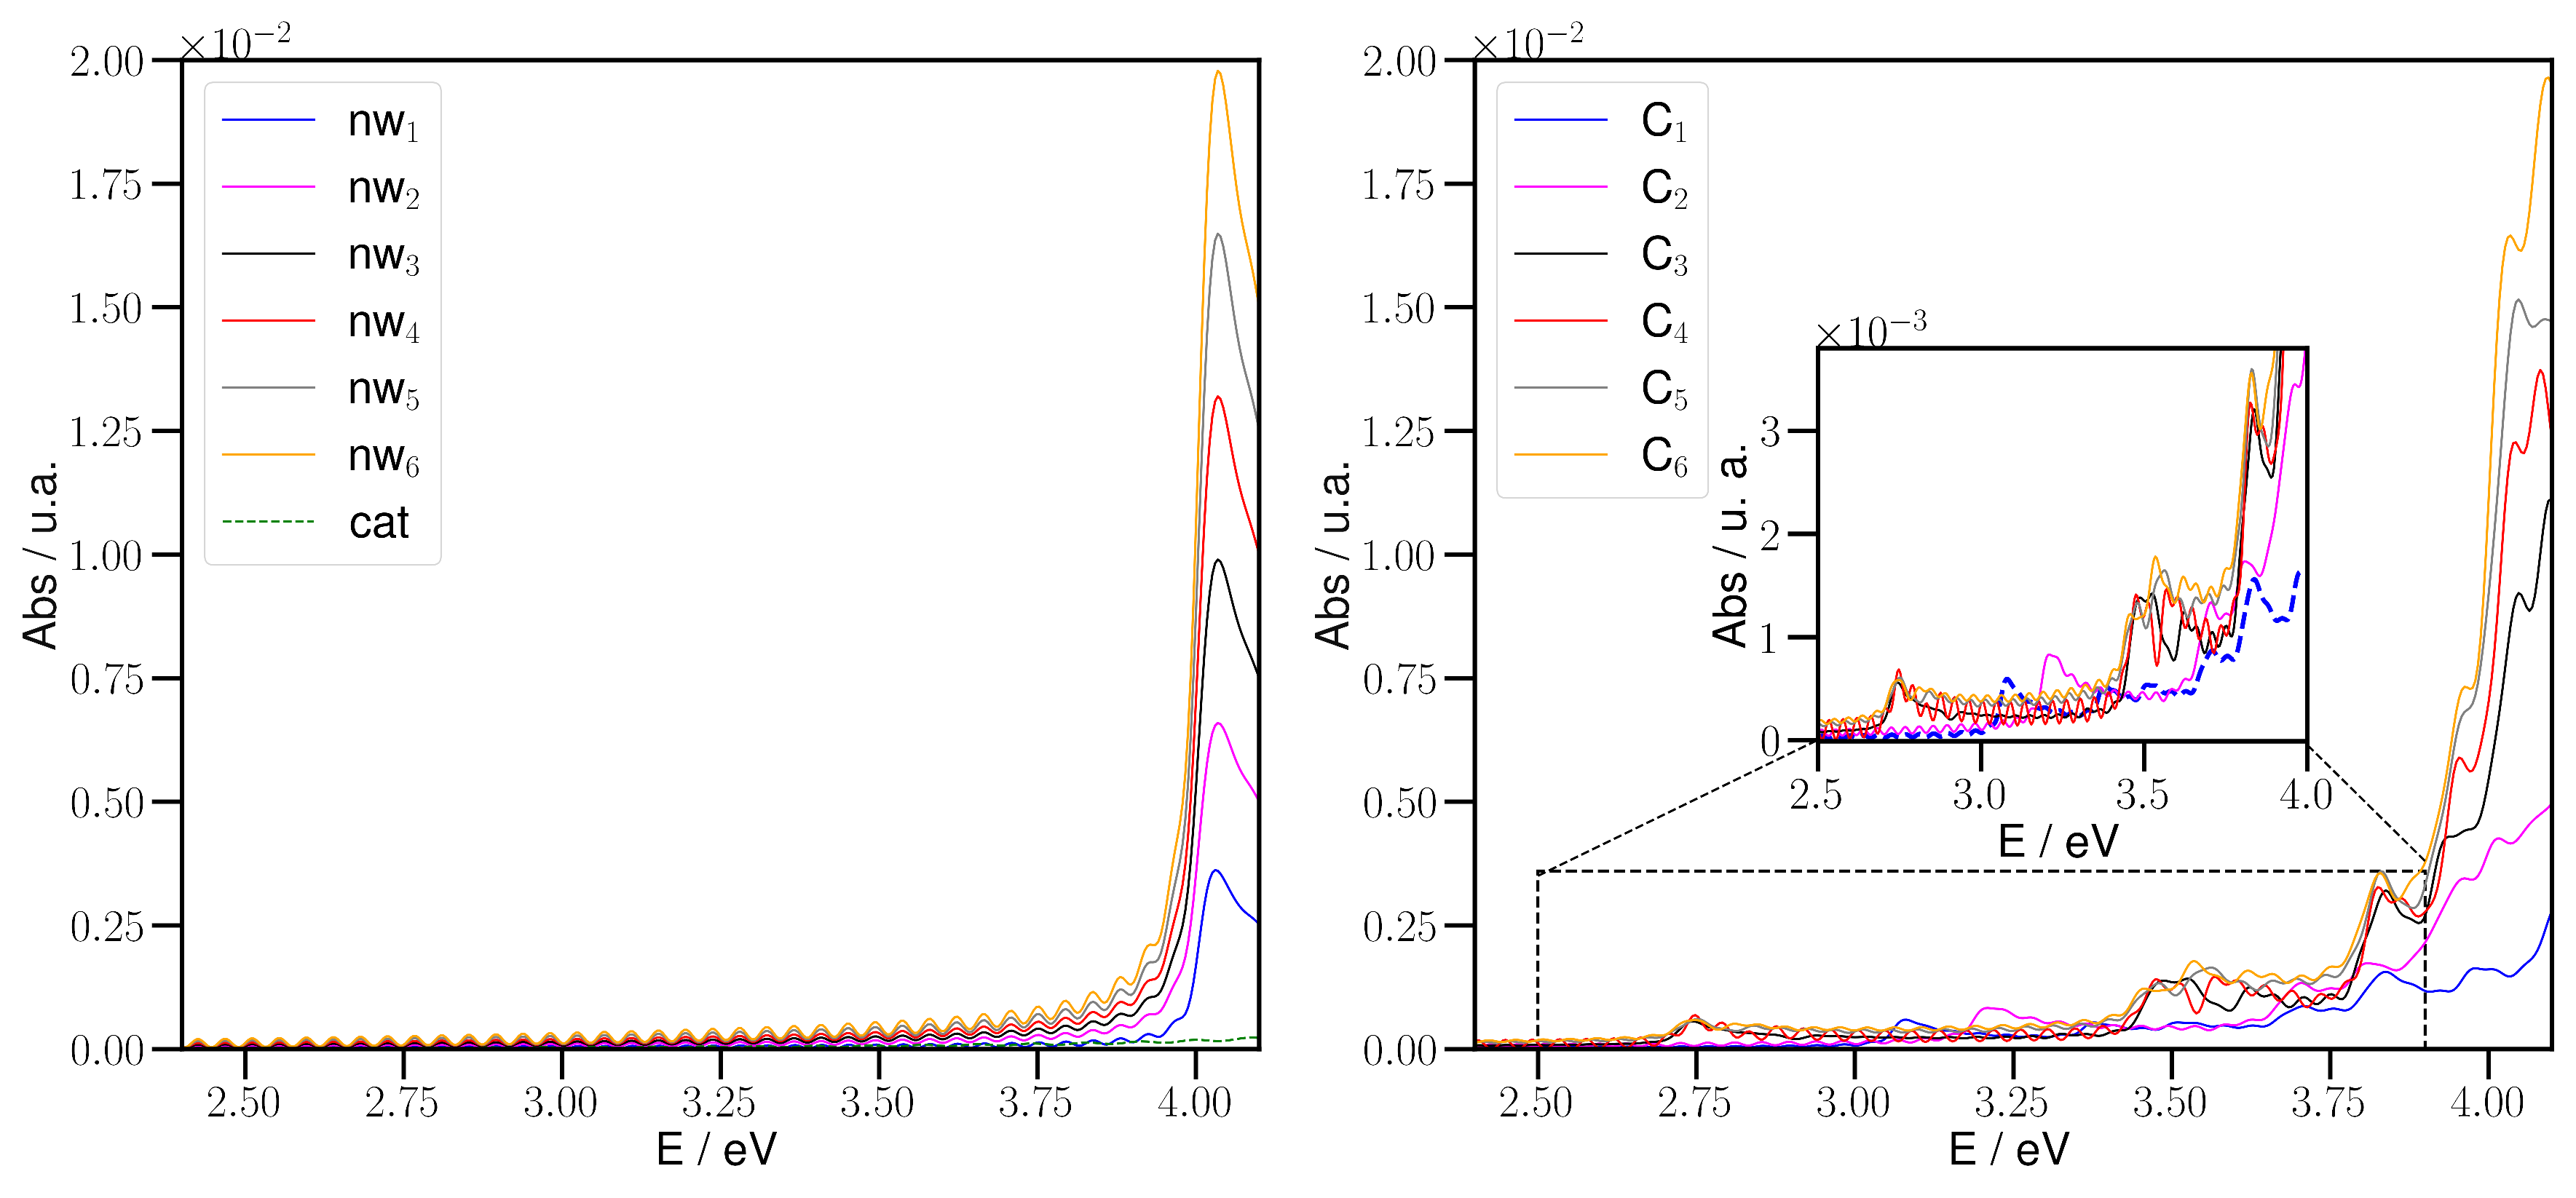
\includegraphics[height=6.5cm]{cap5/fig/specs.eps}
\caption{Espectros de absorción simulados con dftb+ ({\bf izquierda}) nw$_x$ y CAT aislado ({\bf derecha}) complejos C$_x$}
\label{specs}
\end{figure}

Si nos enfocamos solo en las bandas de menor energía para cada complejo, observamos que C$_3$, C$_4$, C$_5$ y C$_6$ tienen el máximo de absorción en $2.7$ eV, $C_1$ en $3.08$ eV y C$_2$ en $3.2$ eV. Estos resultados nos muestran que tanto el catecol como los nw son transparentes a la luz visible cuando se encuentran separados. Sin embargo, la absorción de la molécula a la superficie del SC genera transiciones en el rango visible como es el caso de los sistemas C$_1$, C$_3$, C$_4$, C$_5$ y C$_6$ o en el límite UV-visible para C$_2$. 
     
Existe un intereés particular en C$_1$ (línea punteada de la figura \ref{specs}), debido a que presenta la E$_{ad}$ más negativa y por ende es el sistema con la unión CAT-nw más fuerte. Por esta razón, a continuación se plantea un análisis más profundo de este complejo. En primer lugar se presentan todos los gráficos de estructura electrónica en el equilibrio como son los cálculos de densidades de estado y estructura de bandas para este sistema junto con los espectros de absorción tal como muestra la figura \ref{dos_bandas_spec}. El conjunto de resultado ayudará a la comprensión de las transiciones que ocurren. 

\begin{figure}[!htb]
\centering
\includegraphics[height=5.7cm]{cap5/fig/dos_bandas_spec.eps}
\caption{(1) DOS C$_1$, pdos de CAT y nw$_1$, (2) Estructura de bandas para C$_1$, (3) Espectros de absorción de: C$_1$, nw$_1$ y CAT, (4) DOS nw$_1$ aislado y (5) Estructura de bandas del nw$_1$ aislado}
\label{dos_bandas_spec}
\end{figure}

En la figura \ref{dos_bandas_spec} (1) y (4) se muestran los cálculos de densidades de estados, en el primero la densidad de estados total (DOS) para C$_1$ y la densidad de estados proyectada ({\bf pdos}) del catecol y el nw$_1$ mientras que en el segundo la DOS del nw$_1$. La estructura de bandas para C$_1$ y nw$_1$, se observan en (2) y (5), respectivamente, y en el medio, los espectros de absorción de CAT y nw$_1$ aislados y C$_1$.      
  
La densidad de estados por unidad de volumen (o simplemente densidad de estados) en un cristal perfecto donde el potencial tiene la periodicidad de la red de Bravais subyacente tiene la forma:

\begin{equation}
\displaystyle g(E) =  \sum_{n} g_n(E), 
\label{eq:dos}
\end{equation}

donde la densidad de estados DOS(E) de la n-ésima banda se define como una integral de superficie \cite{Ashcroft76}:

\begin{equation}
\displaystyle DOS(E) =  \int_{S_n(E)} \frac{dS}{4\pi^3} \frac{1}{|\nabla E_n({\bf k})|}, 
\label{eq:dos_n}
\end{equation}

sea E$_n({\bf k})$ la energía de la n-ésima banda para los valores {\bf k} permitidos, S$_n$(E) la porción de la superficie E$_n({\bf k})$=E que se encuentra dentro de la celda primitiva y $\nabla E({\bf k})$ un vector normal a esa superficie cuya magnitud es igual a la tasa de cambio de E$_n({\bf k})$ en la dirección normal. Podemos relacionar los gráficos de densidad de estados y estructura de bandas utilizando la ecuación \ref{eq:dos_n}: E$_n({\bf k})$ es periódica en la red recíproca y en general diferenciable en todas partes y seguramente habrá valores de ${\bf k}$ en cada celda primitiva en los que $\nabla$E = 0. En los máximos y mínimos locales el gradiente es cero y en consecuencia el integrando de la densidad de estados diverge. 


Observamos que la DOS y ambas pDOS de C$_1$ de la figura \ref{dos_bandas_spec}(1) divergen para los valores de energías calculados en el punto G de la estructura de bandas (2) donde la derivada es cero. El gráfico (1) muestra cuáles son las especies que contribuyen con estados a las bandas, el catecol aporta estados a toda la b$_a$ (en $-1.5$ eV) sin dispersión mientras que el nw$_1$ aporta estados al resto de las bandas que tienen dispersión. Estos resultados coinciden con lo que hemos observado al graficar los OM (figura \ref{om}). En el gráfico (4) se observa la DOS del nw aislado con discontinuidades en los máximos y mínimos locales de la estructura de bandas (5).


El espectro de absorción de C$_1$ (3) señala con flechas las nuevas bandas que aparecen al formarse el complejo en el rango ($3-4$) eV. Se puede asignar en la estructura de bandas (2), mediante flechas de colores, cuáles son las transiciones que generan las absorciones en el espectro restando las energías en G entre 2 bandas y comparando esos valores con las energías de los máximos de absorción del espectro. Estas asignaciones se realizaron en G debido a que en este punto ocurren las transiciones de menor energía para cada banda. Por ejemplo, la banda en el espectro con máximo de absorción a $3.08$ eV (flecha negra) se corresponde con la diferencia energética entre el borde de la b$_c$ y la b$_a$, entonces suponemos que la absorción ocurre por la transición mencionada. Sin embargo, es necesario estudiar la naturaleza de las excitaciones de una manera más profunda analizando la evolución temporal de las poblaciones y de las cargas. Estos cálculos se llevaron a cabo perturbando el sistema con un campo eléctrico que oscila en el tiempo. Para ello se realizaron simulaciones de un láseres continuos sintonizados con las energías de interés, en este caso las energías que analizamos son $3.08$ eV, $3.38$ eV, $3.50$ eV, $3.70$ eV, $3.83$ eV y $3.97$ eV. 

\subsection{Evolución temporal de las cargas de Mulliken y de las poblaciones electrónicas}

\begin{figure}[!htb]
\centering
\includegraphics[height=7.2cm]{cap5/fig/cargas_3.08.eps}

\vspace{0.5cm}

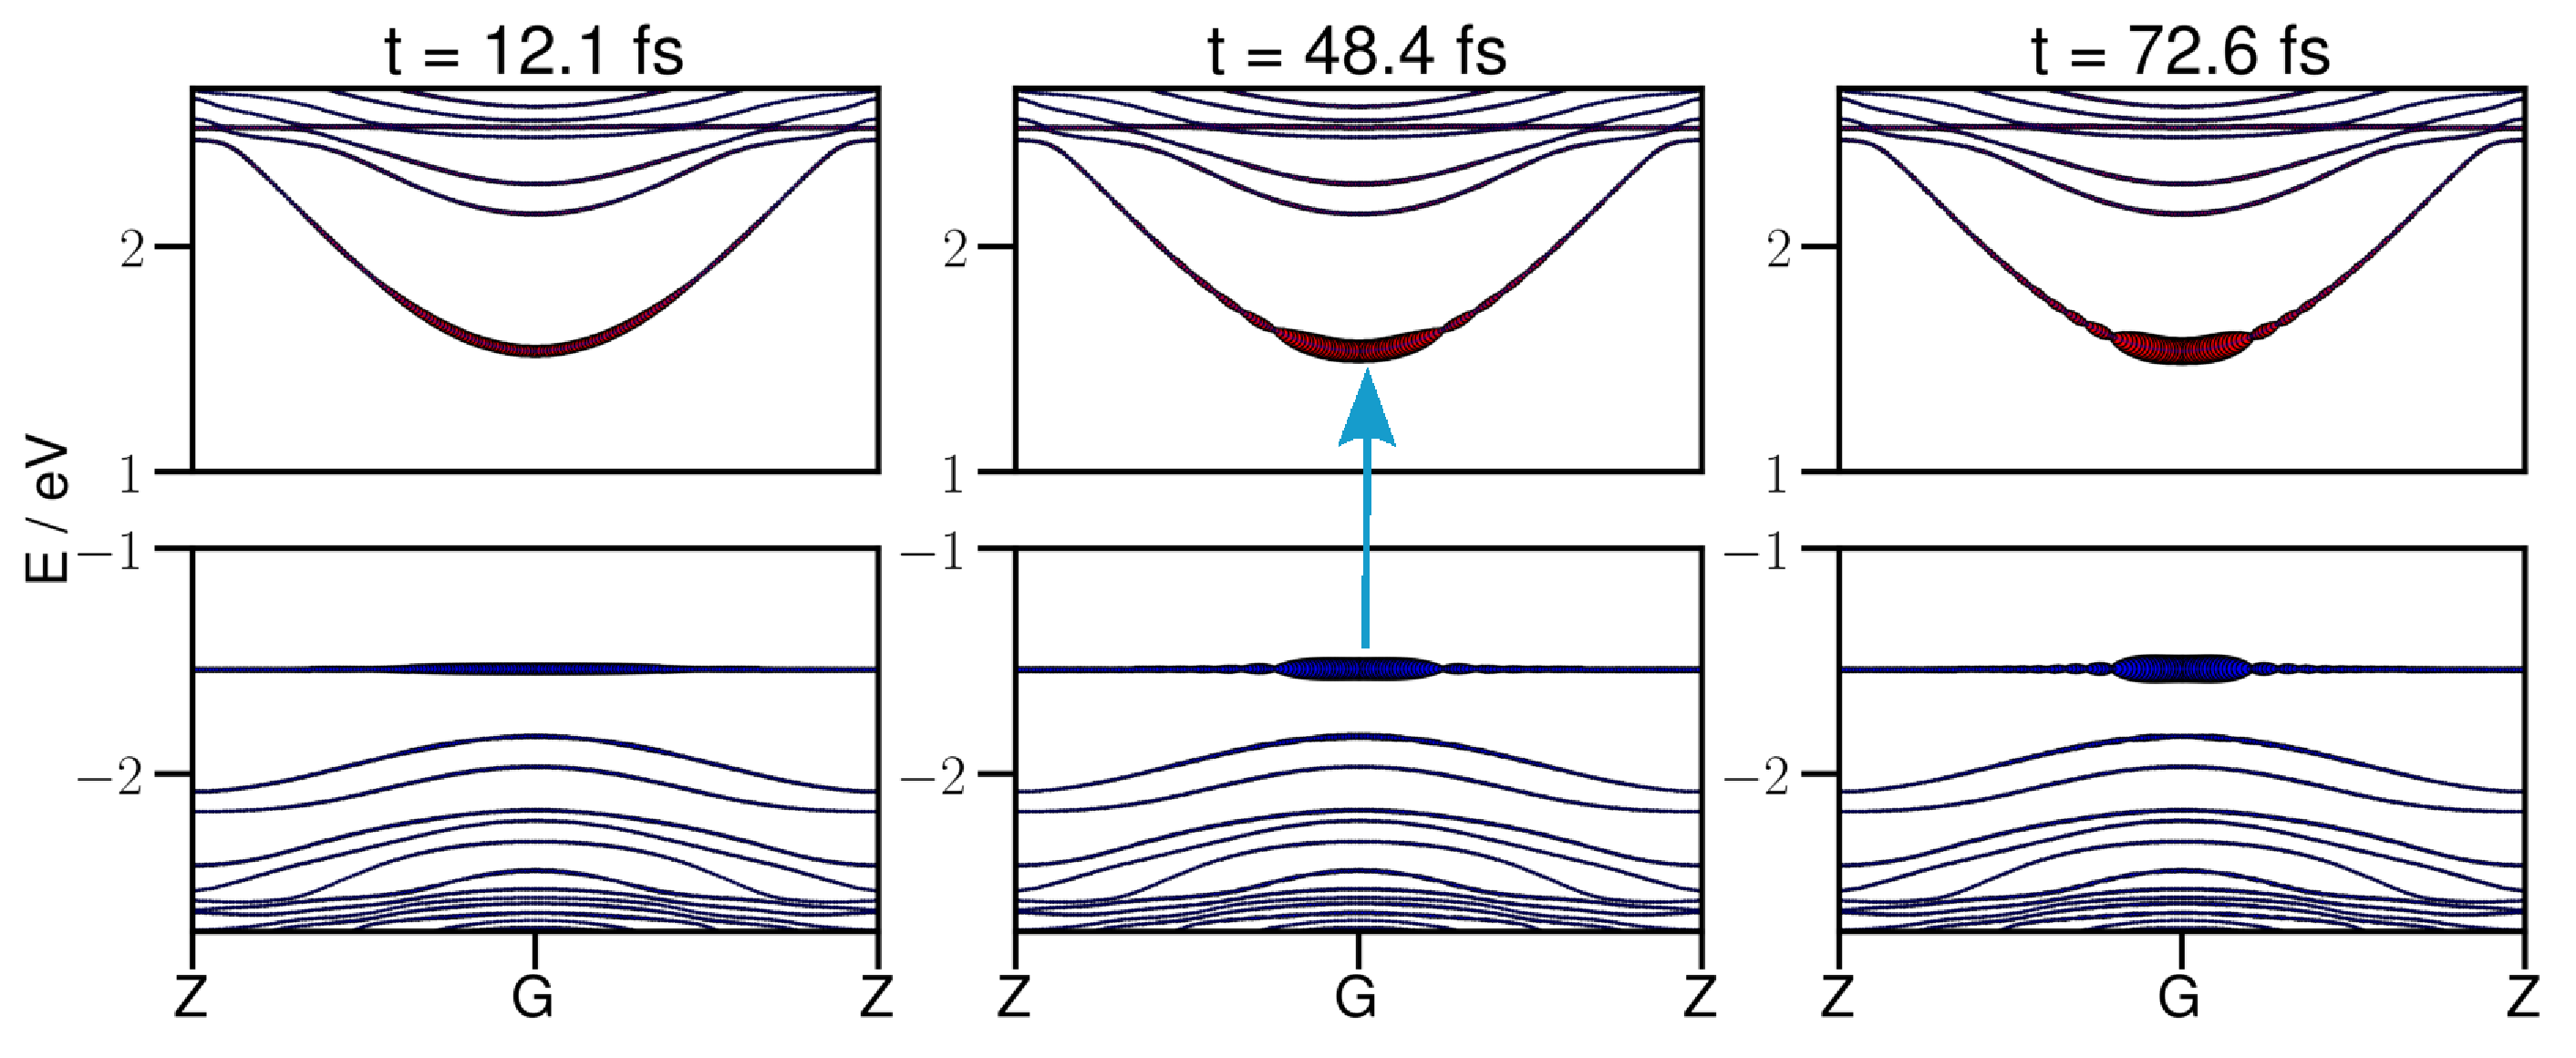
\includegraphics[height=6cm]{cap5/fig/dynpop_3.08_cut.eps}
\caption{ ({\bf Arriba}) izquierda: Espectro de absorción para C$_1$, CAT aislado y nw$_1$ aislado y derecha: cargas en función del tiempo al perturbar el sistema con un láser de $3.08$ eV. ({\bf Abajo}) estructura de bandas de C$_1$. Sobre las bandas se grafica la diferencia de población electrónica que se genera al iluminar C$_1$ con el láser a 3 tiempos distintos: en azul se representa la disminución de la población electrónica al iluminar y en rojo el aumento de la población electrónica al iluminar con el láser.}
\label{ilu_3.08}
\end{figure}


En primer se iluminó el sistema con un láser seteado a $3.08 eV$, es decir con el máximo de absorción de la banda menos energética (como señala la figura \ref{ilu_3.08}) durante $100$ fs. Para obtener información acerca de la evolución temporal de las cargas mientras el complejo C$_1$ es irradiado, se calcularon y graficaron las cargas de Mulliken en el periodo de tiempo mencionado (figura \ref{ilu_3.08} arriba a la derecha). Se observa del gráfico que a medida que transcurre el tiempo el nw va adquiriendo carga negativa (rosa) en la misma medida en la que el catecol (verde) se carga positivamente. Estos resultados indican que los electrones se inyectan desde el catecol a la BC del nw, es decir que la carga se transfiere desde el colorante al SC. Otra observación importante en el gráfico es que la dependencia entre las cargas y el tiempo es prácticamente lineal, lo cual señala que a dinámicas más largas la transferencia seguirá aumentando.  

La figura \ref{ilu_3.08} abajo muestra 3 gráficos de estructura de bandas de C$_1$. Sobre cada uno de ellos se graficó la diferencia de población electrónica que se genera al iluminar con el láser:


\begin{multline}
\Delta P = \textrm{Población electrónica cuando se ilumina con el láser} -  \\
           \textrm{Población electrónica antes de iluminar con el láser}
\end{multline} 


cuando $\Delta P$ es positivo, la población electrónica aumenta con la irradiación mientras que cuando $\Delta P$ arroja un valor negativo, la población electrónica disminuye. En los gráficos se muestran los valores de $\Delta P$ tomados en 3 tiempos distintos de la dinámica y se representa en rojo la diferencia de población positiva ($\Delta P$+) y en azul la diferencia de población negativa ($\Delta P$-).


A tiempos cortos ($12.1$ fs) el láser no llega a aportar la energía necesaria para generar una diferencia de población y en consecuencia se produzca la transición, en ese momento todas las transiciones son posibles. A medida que transcurre el tiempo, por ejemplo a la mitad de la dinámica ($48.4$ fs) se observa la disminución de población en b$_a$ a $-1.5$ eV y aumento en la banda menos energética de la BC, es decir b$_1$ (ver figura \ref{comp_bandas}). En el punto G (en ambas bandas) es donde se produce la mayor $\Delta P$ y por eso es allí donde ocurre la transición (flecha de color celeste). Tan pronto nos alejamos del centro de la ZB, $\Delta P$ comienza a disminuir y se observa la presencia de nodos (donde la $\Delta P$ = 0) a medida que esto ocurre. A tiempos más largos ($72.6$ fs), la transición observada es la misma pero la población electrónica cambia, $\Delta P$ se va localizando cada vez más en G y los nodos se muestran para valores diferentes de ${\bf k}$ con respecto al caso anterior. 

Los resultados obtenidos en los gráficos se puede explicar mediante la Regla de Oro de Fermi o la Regla de Oro de la Teoría de Perturbaciones dependiente del tiempo, la cual aplica la teoría perturbaciones dependiente del tiempo a un sistema que sufre una transición desde un estado inicial $\ket i$ a un estado final $\ket f$ que es parte de un continuo de estados es decir, cuando la energía pertenece a una parte continua del espectro de H$_0$ (hamiltoniano del sistema sin perturbar), entonces debemos tener en cuenta todos los estados a los que el sistema puede saltar. 
Para una gran cantidad de problemas, es suficiente la teoría de la perturbación independiente del tiempo. Sin embargo, hay casos en los que queremos estudiar cómo los sistemas responden a las perturbaciones impuestas y luego se establecen en estados estacionarios después de un intervalo, es decir, estudiar las transiciones inducidas por una perturbación entre estados estacionarios del sistema no perturbado. En casos como estos, utilizamos la teoría de la perturbación dependiente del tiempo para calcular, entre otras cosas, las probabilidades de transición. La ecuación de Schr\"odinger dependiente del tiempo para el sistema es \cite{Koukaras}: 

\begin{equation}
\displaystyle H \ket {\Psi (t)} = [H_0 + W(t)]  \ket {\Psi (t)} =  i \hbar \frac{\partial \ket {\Psi (t)}}{\partial t} 
\label{eq:sch_dep_t}
\end{equation}


donde se asume que el hamiltoniano H del sistema puede ser escrito de la forma $H = H_0 + W(t)$ donde $W(t)$ es la perturbación aplicada al sistema y que el estado del sistema $\ket {\Psi}$  al tiempo t, se expresa como una combinación lineal de las funciones base ${\phi_n}$: 


\begin{equation}
\displaystyle \ket {\Psi (t)} = \sum_n c_n(t) \ket {\Psi_n (t)} = \sum_n c_n(t) \ket {\phi_n (t)} e^{\frac{-i E_n(t)}{\hbar}}   
\label{eq:base}
\end{equation}


Las funciones base $\phi_n$ provienen de la ecuación de Schr\"odinger independiente del tiempo del sistema sin perturbar ($H_0 \phi_n  = E_n \phi_n$) y están relacionadas con las funciones de onda no perturbadas dependientes del tiempo por

\begin{equation}
\displaystyle \ket {\Psi_n (t)} = \ket {\phi_n (t)} e^{\frac{-i E_n(t)}{\hbar}}   
\label{eq:relaciones_func_onda}
\end{equation}

Al insertar la relación \ref{eq:base} en \ref{eq:sch_dep_t} y proyectando el resultado en $\phi_n$ obtenemos:

\begin{equation}
\displaystyle    \frac{\partial c_n(t)}{\partial t}  = \frac{1}{i\hbar} \sum_k c_k(t) W_{nk} (t) e^{i w_{nk} t)}
\label{eq:coeff_s_aprox}
\end{equation}

donde $W_{nk} = \bra {\phi_n} W(t) \ket {\phi_k}$ son los elementos de matriz de la perturbación y $w_{nk}$ es $\frac{E_n-E_k}{\hbar}$

Para evaluar los coeficientes de \ref{eq:coeff_s_aprox} suponemos que: {\bf (a)} el sistema está inicialmente en el estado $\ket{i}$, por lo tanto, todos los coeficientes en t = 0 son iguales a cero, excepto para $c_i$: $c_j$ (t = 0) = $\delta_{ij}$ y {\bf (b)} la perturbación es muy débil y se aplica durante un corto período de tiempo, de modo que todos los coeficientes permanecen casi sin cambios. Entonces la ecuación \ref{eq:coeff_s_aprox} ahora se transforma en:


\begin{equation}
\displaystyle \frac{\partial c_n(t)}{\partial t} = \frac{1}{i\hbar} c_i(t) W_{ni} (t) e^{i w_{ni} t)}
\label{eq:coeff_c_aprox}
\end{equation}

así que para cualquier estado final el coeficiente será: 

\begin{equation}
\displaystyle \frac{\partial c_n(t)}{\partial t} = \frac{1}{i\hbar} \int_0^t W_{fi} (t') e^{i w_{fi} t')} dt'
\label{eq:coeff_final}
\end{equation}

La aplicación de la perturbación cambia el estado del sistema desde el estado inicial $\ket{\phi_i}$ a un estado final $\ket{\phi_f}$, ambos son estados propios del hamiltoniano no perturbado H$_0$. La probabilidad de encontrar el sistema en el estado propio $\ket{\phi_f}$ es: 


\begin{equation}
\displaystyle P_{if}(t) = {|\langle\phi_f |\psi(t) \rangle |}^2
\label{eq:prob_1}
\end{equation}

y utilizando \ref{eq:coeff_final} obtenemos:

\begin{equation}
\displaystyle P_{if}(t) = \frac{1}{\hbar^2} \left| \int_0^t W_{fi} (t') e^{i w_{fi} t')} dt'\right |^2
\label{eq:prob_2}
\end{equation}

Una perturbación oscilante (como un láser) está definida de la forma:

\begin{equation}
\displaystyle W(t) = 2 W \cos(wt) = 2 (e^{i w t} + e^{-i w t})
\label{eq:pert_laser}
\end{equation}

Insertando esta ecuación en \ref{eq:coeff_final} obtenemos:


\begin{align}
\displaystyle c_f(t) &= \frac{W_{fi}}{i\hbar} \left\lbrace\frac{e^{i(w_{fi} + w) t)}-1}{i (w_{fi} + w)} + \frac{e^{i (w_{fi} - w) t)}-1}{i (w_{fi} - w)}\right\rbrace
\label{eq:coeff_final_oscilante}
\end{align}


Entonces la ecuación \ref{eq:prob_2} se transforma en (e introduciendo la función $F(t,w-w_{fi}$):


\begin{align}
\displaystyle P_{if}(t) &= \frac{W_{fi}^2}{\hbar^2} \left|\frac{e^{i(w_{fi} + w) t)}-1}{i (w_{fi} + w)} + \frac{e^{i (w_{fi} - w) t)}-1}{i (w_{fi} - w)}\right|^2  \\
&= \frac{W_{fi}^2}{\hbar^2} F(t,w-w_{fi})
\label{eq:prob_final}
\end{align}

Cuando el estado final es parte de un continuo de estados la probabilidad se obtiene integrando la probabilidad dada por la ecuación \ref{eq:prob_final} con la densidad de estados $\rho(E)$ como peso: 


\begin{equation}
\displaystyle P(t) = \int_{Eacc} P_{if}(t) \rho(E) dE
\label{eq:prob_osc}
\end{equation}

donde ${Eacc}$ denota todos los estados a los que el sistema puede saltar bajo la influencia de la perturbación. Sustituyendo \ref{eq:prob_final} en \ref{eq:prob_osc} obtenemos:

\begin{equation}
\displaystyle P(t) = \int_{Eacc} \frac{W_{fi}^2}{\hbar^2} F(t,w-w_{fi}) \rho(E) dE
\end{equation}

como el rango de energías es muy estrecho, el elemento de matriz $W_{fi}$ y la densidad de estados $\rho(E)$ se pueden considerar como constantes. Entonces la probabilidad es una integral de $F(t, w-wfi)$:

\begin{equation}
\displaystyle P(t) = \frac{W_{fi}^2}{\hbar^2} \rho(E) \int_{Eacc} F(t,w-w_{fi})dE
\label{eq:prob_osc_final}
\end{equation}


En la figura \ref{fermi_F} se observa un gráfico de $F(t,w)$ en función de w, a 4 tiempos distintos, donde $t1<t2<t3<t4$

\begin{figure}[!htb]
\centering
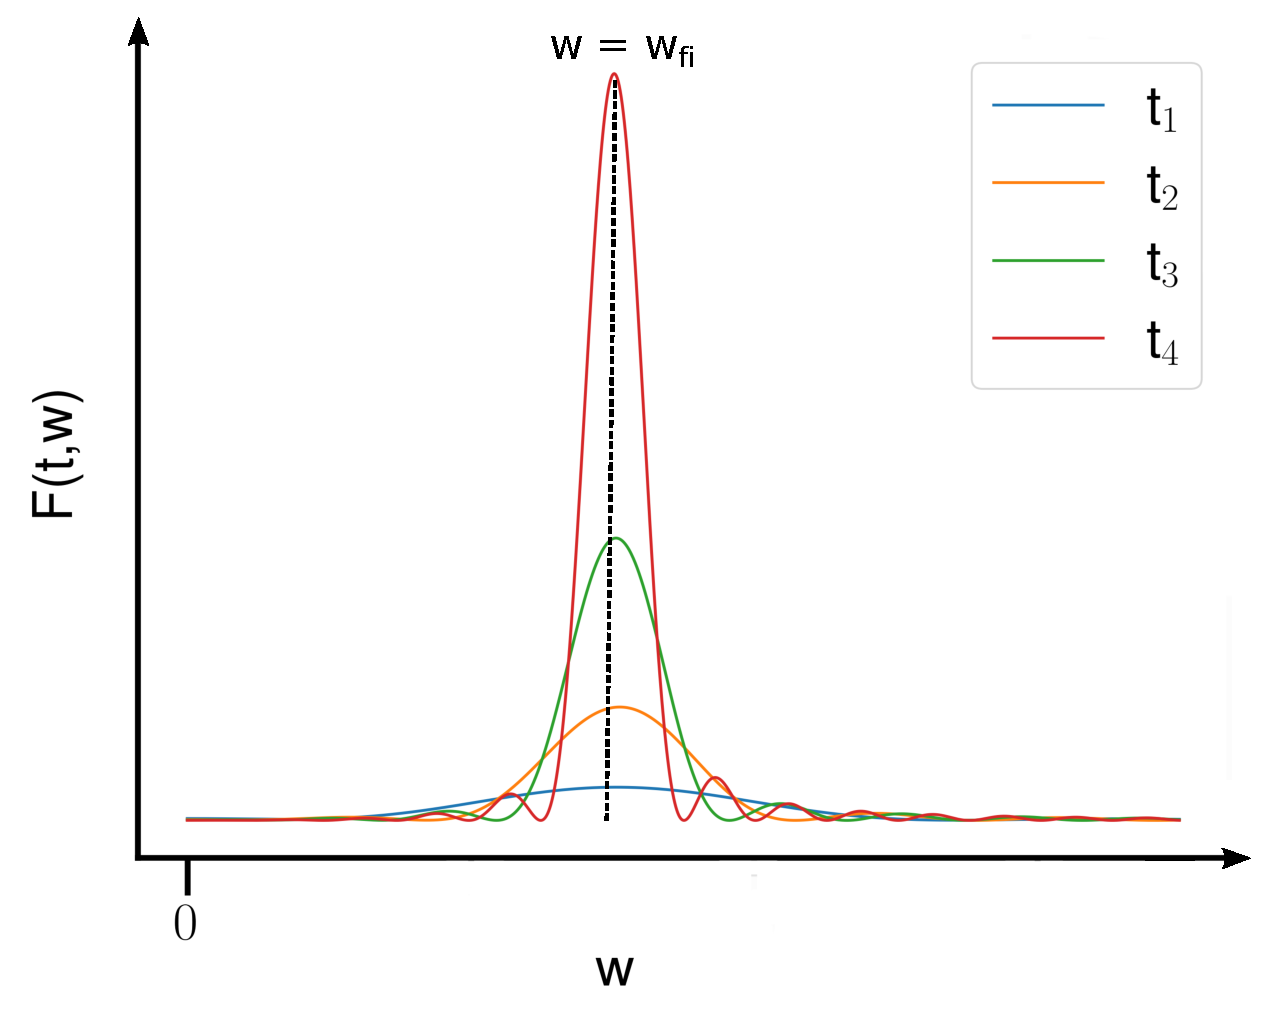
\includegraphics[height=7.8cm]{cap5/fig/fig_nodos_cut.eps}
\caption{$F(t,w)$ vs w, donde $F(t,w)$ actúa como una función delta de Dirac para 4 tiempos donde $t1<t2<t3<t4$´}
\label{fermi_F}
\end{figure}


Los cuatro gráficos representan a $F(t,w)$ como una función con un pico centrado en $w = w_{fi}= \frac{E_f-E_i}{\hbar}$ y valores de w donde $F(t,w) = 0$ o la probabilidad es cero (nodos). A medida que el sistema evoluciona temporalmente, la función se va haciendo más aguda en w$_{fi}$, es decir que en t=$\inf$ F es una función delta de Dirac. Simultáneamente, los nodos toman valores que se van acercando cada vez más a w$_{fi}$.


$F(t,w)$ justifica entonces la concentración de $\Delta P$ en la frecuencia de resonancia (que se muestra en G) con el aumento del tiempo, tal como se observó en la figura \ref{ilu_3.08}. Luego, al graficar las diferencias de poblaciones electrónicas a los 4 tiempos mencionados anteriormente utilizando la Regla de Oro de Fermi encontramos que el modelo planteado representa cualitativamente los cálculos obtenidos con dftb+ (ver figura \ref{fermi_bandas}). 


\begin{figure}[!htb]
\centering
\subfloat[t$_1$]{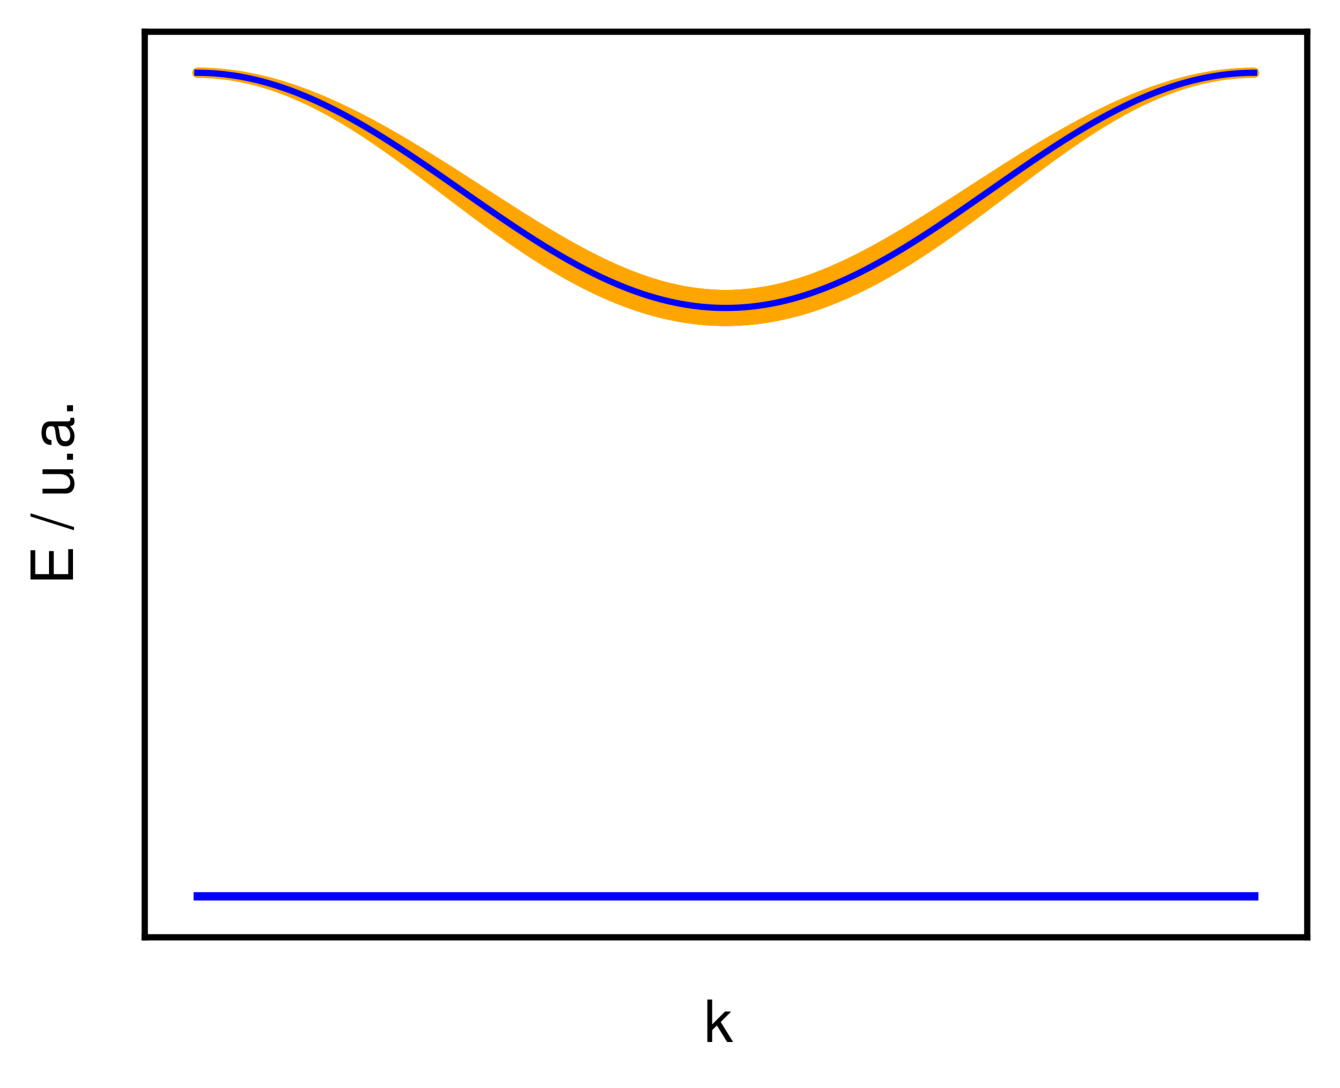
\includegraphics[height=6cm]{cap5/fig/fig_time1.eps}}
\subfloat[t$_2$]{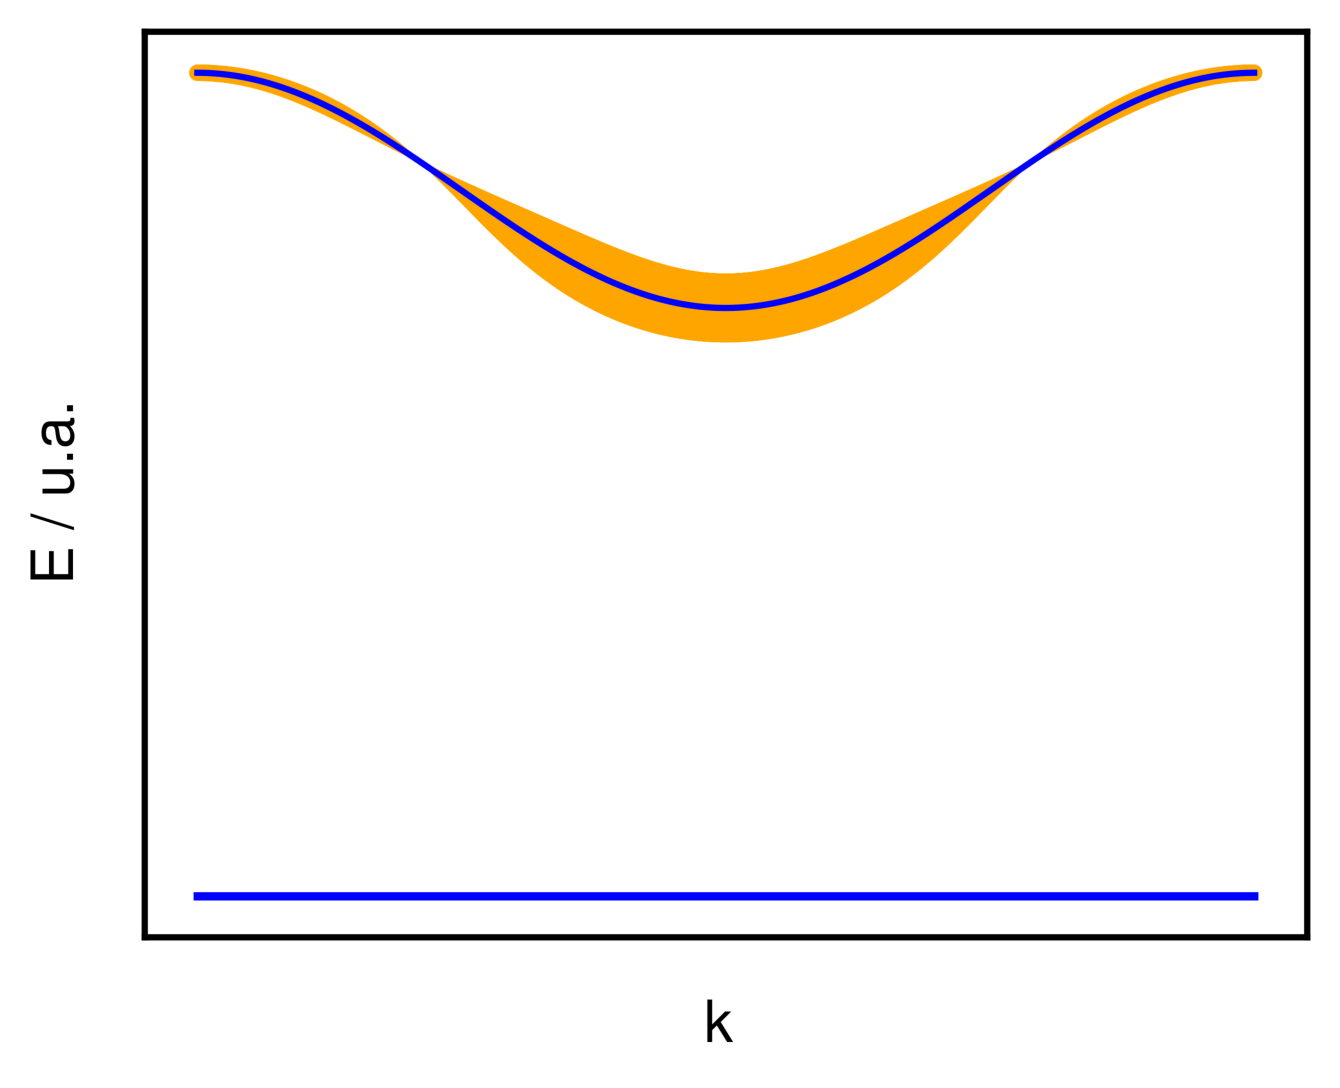
\includegraphics[height=6cm]{cap5/fig/fig_time2.eps}}


\subfloat[t$_3$]{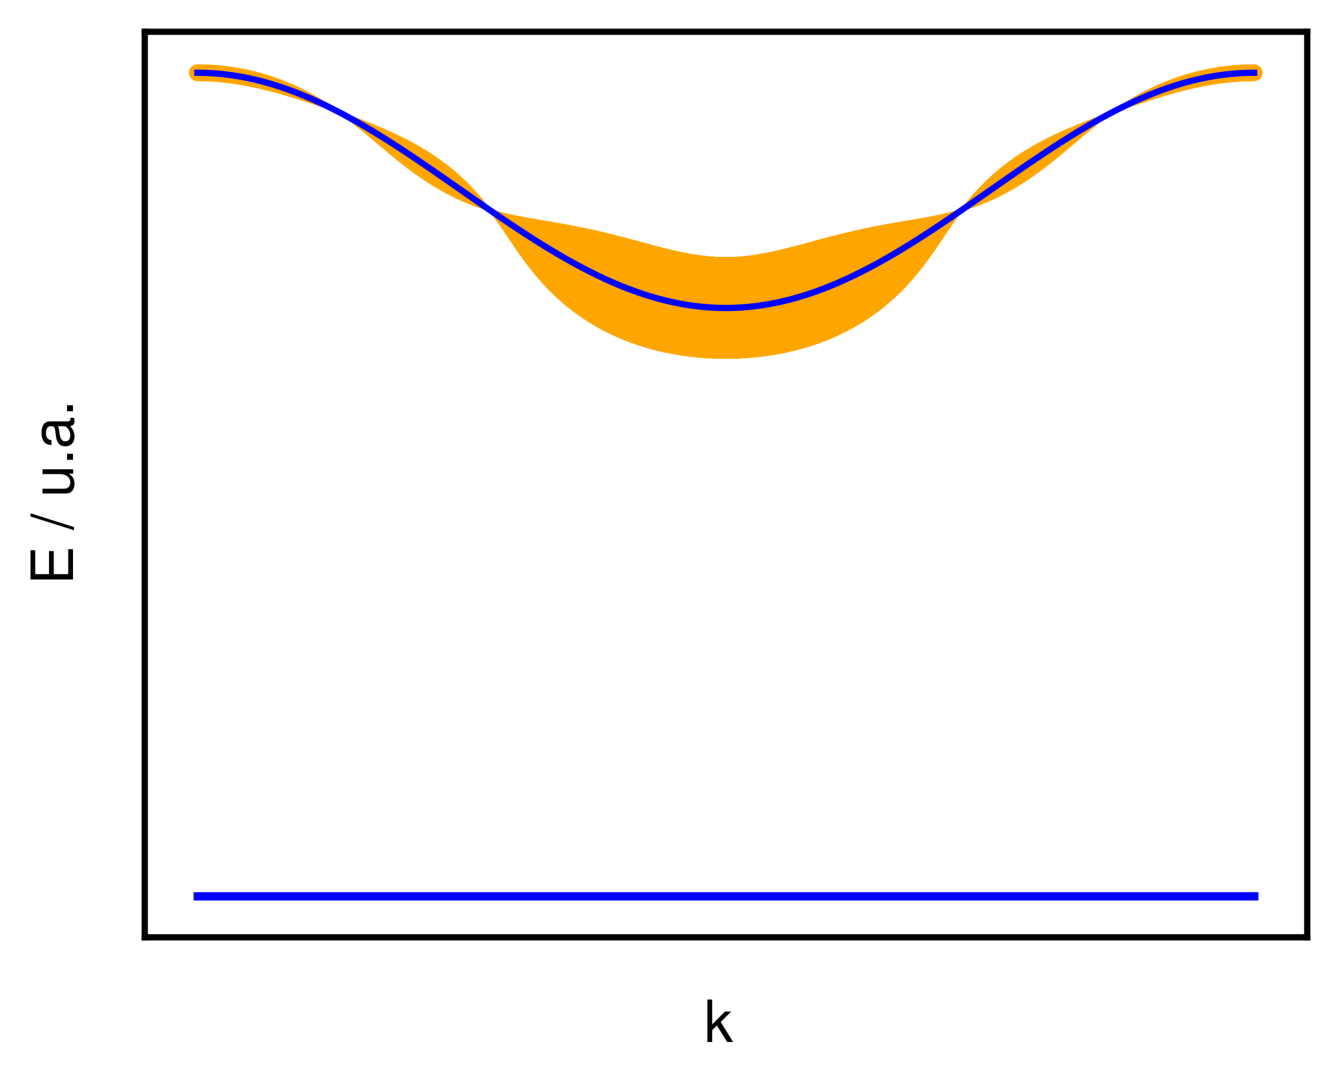
\includegraphics[height=6cm]{cap5/fig/fig_time3.eps}}
\subfloat[t$_4$]{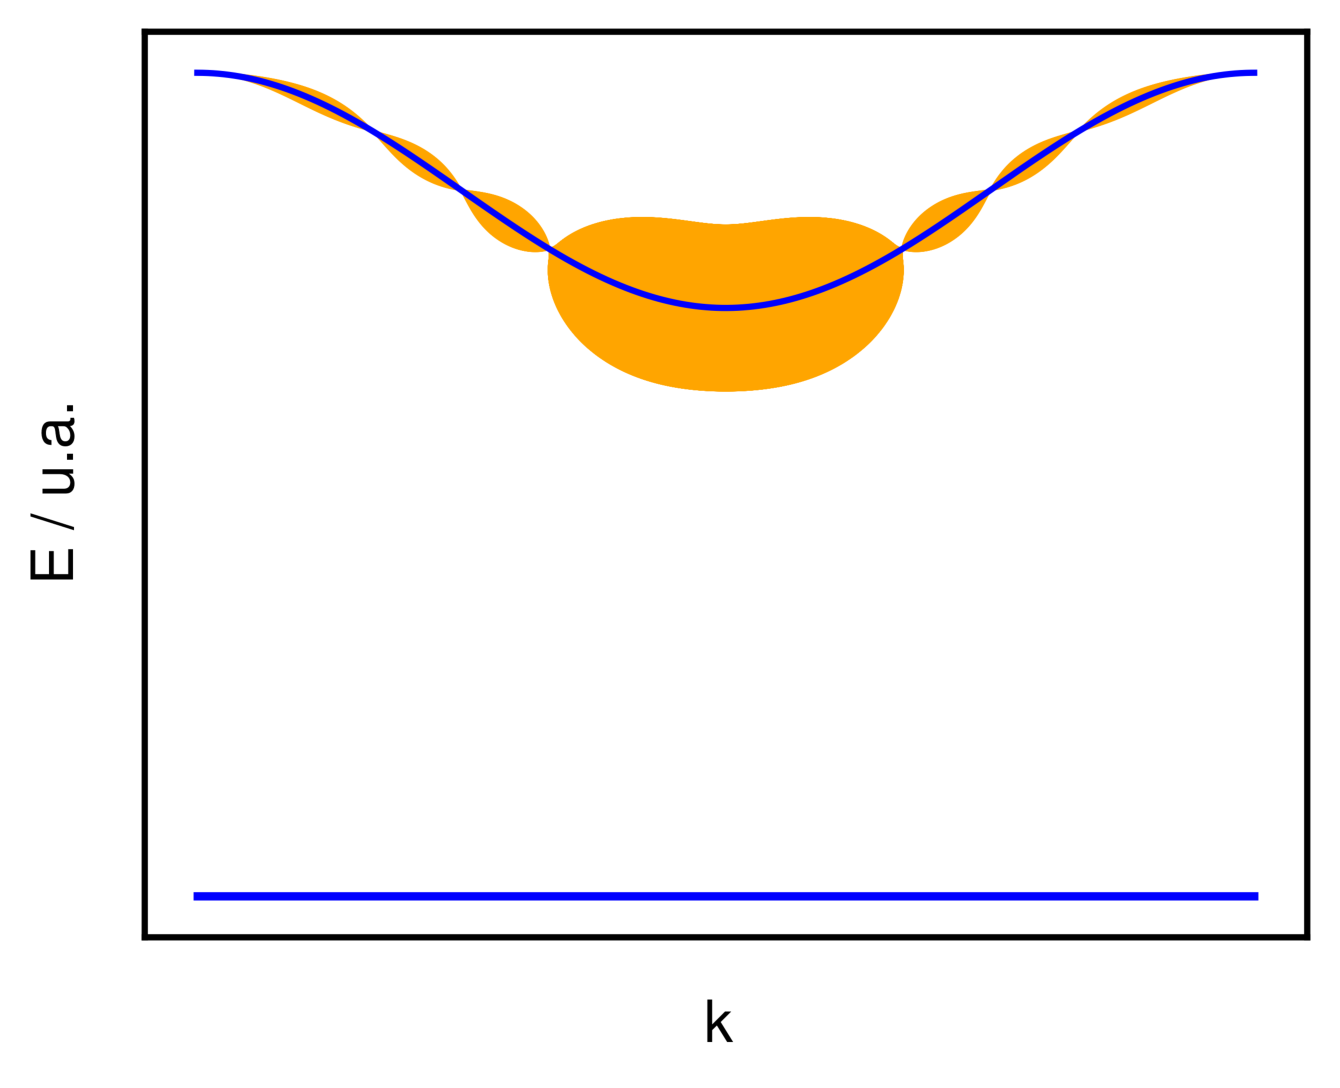
\includegraphics[height=6cm]{cap5/fig/fig_time4.eps}}
\caption{Estructura de bandas (azul) y $\Delta P$ (naranja) cuando el estado final es parte de un continuo de estados de acuerdo a la Regla de Oro de Fermi para 4 tiempos, donde $t1<t2<t3<t4$}
\label{fermi_bandas}
\end{figure}

Estos resultados, los cuáles obedecen la regla de oro de Fermi, no sólo permite explicar la evolución de las poblaciones electrónicas simuladas cuando iluminamos C$_1$ con un láser sintonizado a $3.08$ eV sino que también permite explicar la relación entre las transiciones que ocurren y la transferencia de carga. En ese caso, la transición más probable se produce en G y es la responsable de la banda a $3.08$ eV del espectro de absorción y de la transferencia de carga entre el colorante y el nw$_1$ debido a que ocurre entre una banda molecular del CAT y otra con mayores contribuciones por parte del SC. Es importante recalcar que la regla de oro de Fermi se ve reflejada en todas las iluminaciones analizadas. 


\begin{figure}[!htb]
\centering
\includegraphics[height=7.2cm]{cap5/fig/cargas_3.38.eps}

\vspace{0.5cm}

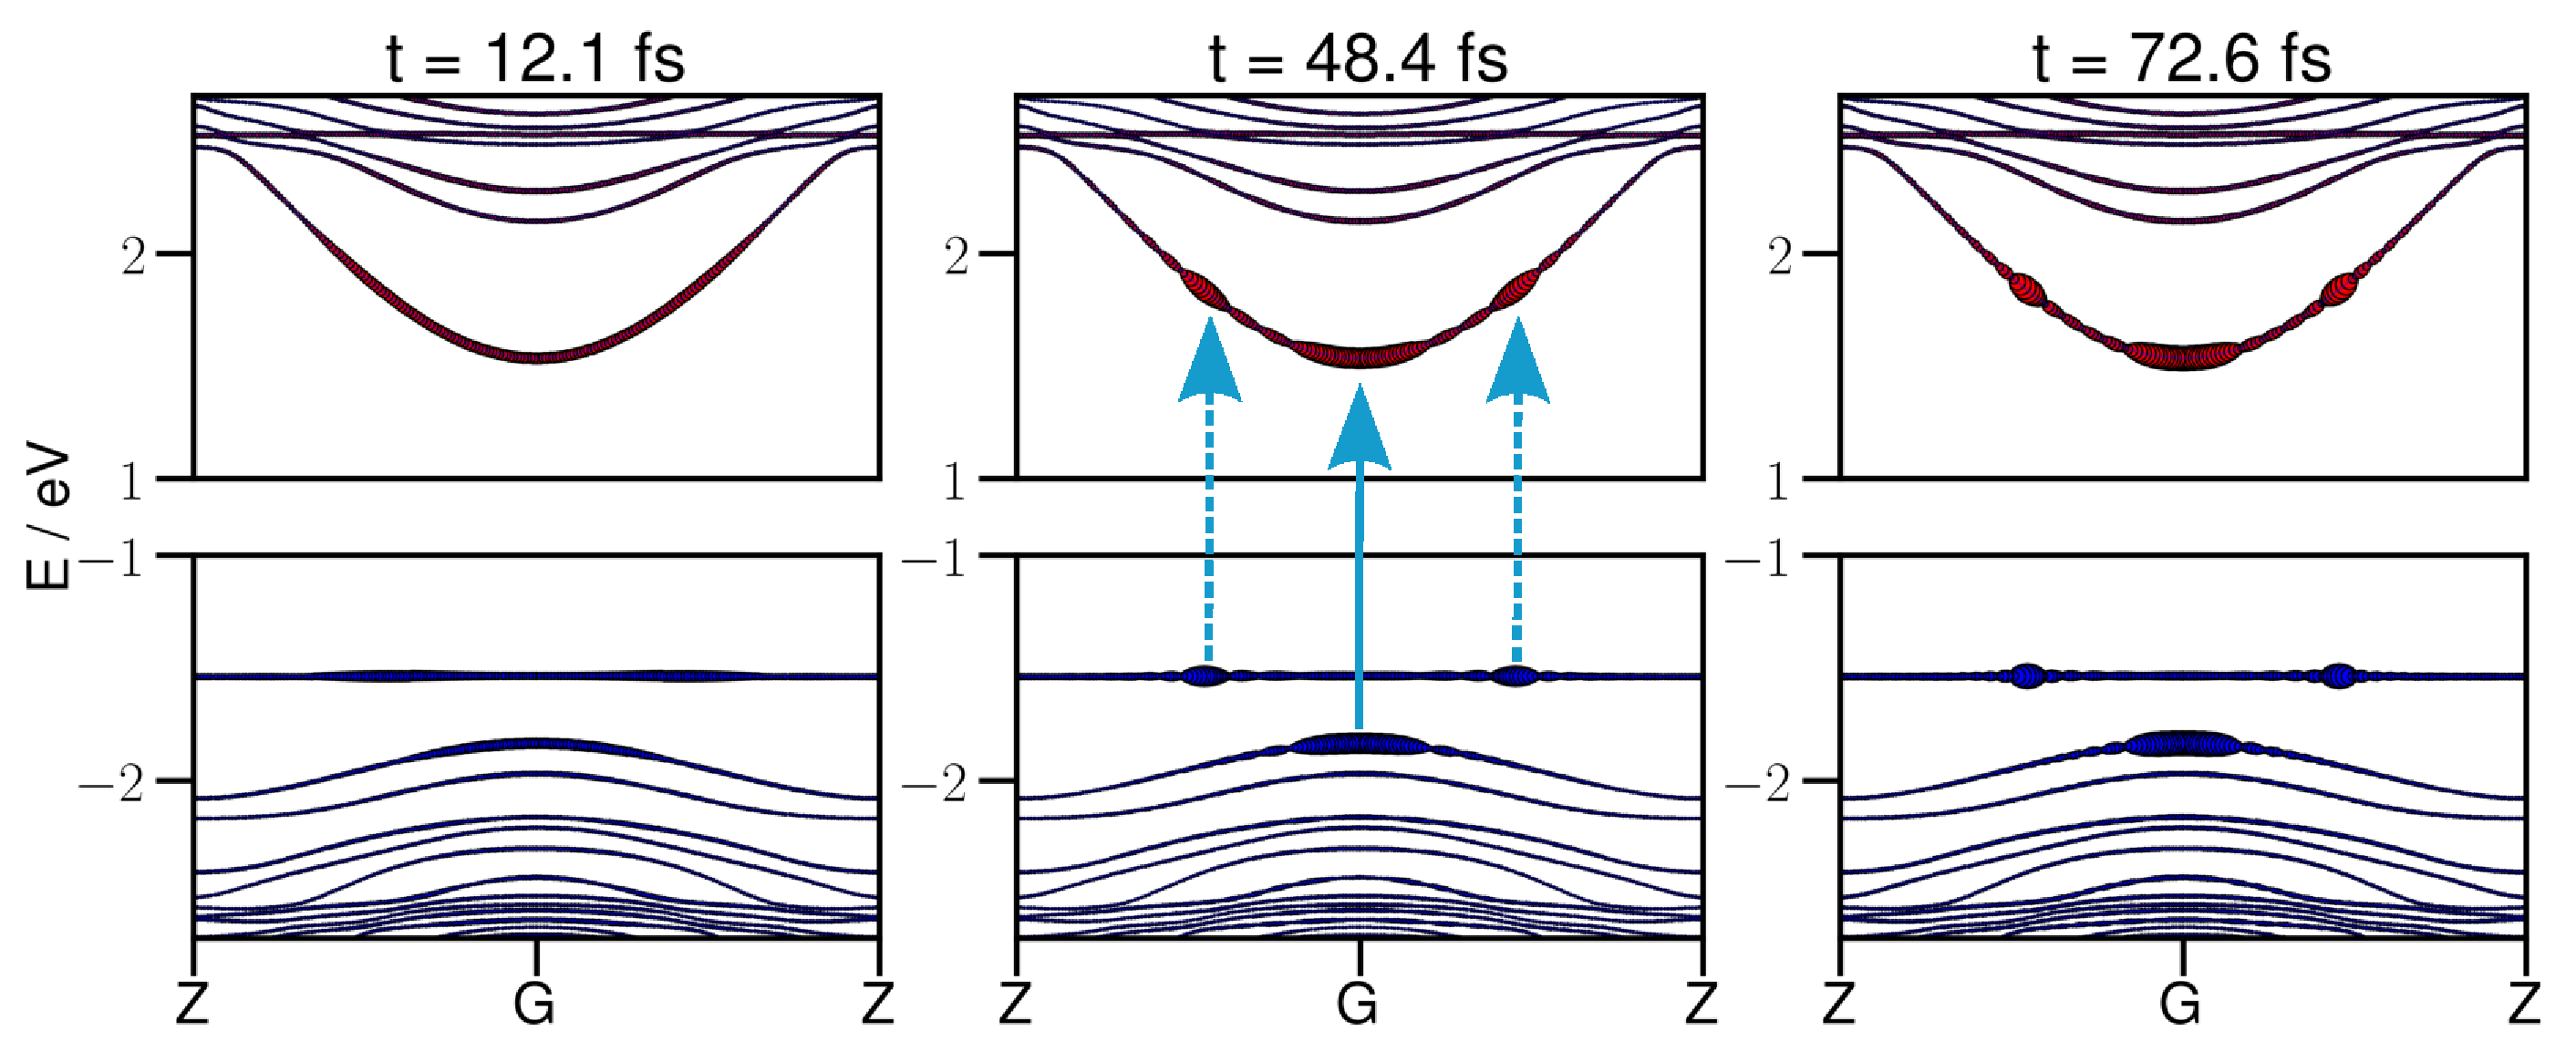
\includegraphics[height=6cm]{cap5/fig/dynpop_3.38_cut.eps}
\caption{ ({\bf Arriba}) izquierda: espectro de absorción para C$_1$, cat aislado y nw$_1$ aislado y  derecha: cargas en función del tiempo perturbando el sistema con un láser de $3.38$ eV. ({\bf Abajo}) Estructura de bandas de C$_1$. Sobre las bandas se grafica la diferencia de población electrónica que se genera al iluminar C$_1$ con el láser a 3 tiempos distintos: en azul se representa la disminución de la población electrónica al iluminar y en rojo el aumento de la población electrónica al iluminar con el láser.}
\label{ilu_3.38}
\end{figure}


Al iluminar C$_1$ con un láser seteado con la energía del máximo de absorción de la segunda banda, es decir a $3.38$ eV (ver figura \ref{ilu_3.38}) no se observa transferencia de carga entre CAT y el nw aunque las transiciones estén presentes tal como lo indica el espectro. Para entender este hecho nos remitimos a los gráficos de $\Delta P$ sobre las bandas, en el cual observamos varias transiciones: a) una transición en G que ocurre entre la b$_b$ y b$_1$, ambas bandas con contribuciones del nw$_1$ (fijarse figura \ref{dos_bandas_spec} (1) y (2)) y b) 2 transiciones una a cada lado de G, entre G y el punto crítico Z que ocurren entre la b$_a$ y b$_1$. En este último caso, las mismas provienen de las excitaciones que se produjeron en el máximo de absorción de la banda de menos energía ($3.08$ eV). La transición en G no contribuye a la transferencia de carga ya que se da entre 2 bandas con mayores contribuciones por parte del nw$_1$ mientras que las otras dos transiciones si contribuyen como se observó en la iluminación anterior. La resultante de las transiciones que ocurren da como resultado final la ausencia de la transferencia de carga. 


%VER ESTA PARTE%

%En general, las bandas que se observan en el espectro son el resultado de las transiciones que ocurren de acuerdo a la ecuación \ref{eq:prob_osc_final} la cual señala que la probabilidad de la transición está directamente relacionada con la integral de $F(t,w)$ entonces calculando el área bajo la curva de esta función centrada en w$_{fi}$ podemos justificar los resultados obtenidos por dftb+ utilizando la regla de oro de fermi.


%Las transiciones no necesariamente generan transferencia de carga, de acuerdo a los gráficos de $F(w,t)$ (figura \ref{fermi_F}) la probabilidad de transición es mayor en w$_{fi}$ y por ende las excitaciones que ocurren en G deberían a priori tener mayor peso con respecto a otras como se observa en las iluminaciones a $3.08$ eV y $3.38$ eV. Sin embargo, cuando la energía del láser es mayor se observan cada vez más transiciones en otros {\bf k} y por lo tanto las mismas van ganan más peso o igualan a las que ocurren en G. En estos casos, se observa transferencia de carga cuando predominan excitaciones que involucren la b$_a$ que es la banda del colorante y otra banda con contribuciones del nw.


\begin{figure}[!htb]
\centering
\includegraphics[height=17cm]{cap5/fig/ultimas_dynpop.eps}
\caption{Gráficos de: ({\bf izquierda}) estructura de bandas de C$_1$ y $\Delta P$ que se genera al iluminar el sistema con E$_{laser}$ de $3.50$ eV, $3.70$ eV, $3.83$ eV y $3.97$ eV a 3 tiempos distintos: en azul $\Delta P - $ y en rojo $\Delta P + $ donde las flechas punteadas representan las nuevas transiciones y ({\bf derecha}) cargas de Mulliken en función del tiempo correspondientes a cada una de las E$_{laser}$ utilizadas.}
\label{ilu_todas}
\end{figure}


En la figura \ref{ilu_todas} se muestran las evoluciones temporales de las poblaciones (izquierda) y de las cargas de Mulliken (derecha) para las iluminaciones a $3.50$ eV, $3.70$ eV, $3.83$ eV y $3.97$ eV. A medida que aumenta la energía de la irradiación, se observan por un lado nuevas transiciones y por otro, que las excitaciones que provienen de las bandas de menor energía se van acercando cada vez más al punto crítico Z y se alejan de G (fijarse en las flechas celestes). De los cálculos realizados, sólo se observa transferencia de carga para $3.08$ eV, $3.83$ eV y $3.87$ eV, particularmente en $3.83$ eV se transfiere mayor carga con respecto al resto. Si bien en las irradiaciones más energéticas analizadas hay mayores contribuciones para que la transferencia ocurra, en $3.97$ eV aparece una nueva excitación entre 2 bandas con aportes predominantes del nw disminuyendo el resultado final. Es importante recalcar que todas las flechas que representan las excitaciones entre bandas tienen la misma longitud, entonces asignando solo una transición podemos mover la flecha y predecir todas las transiciones que ocurren. Este procedimiento ayuda principalmente al investigar iluminaciones a mayores energías en donde el proceso de asignación es engorroso. 


\section{Conclusiones}

En este capítulo se utilizó como herramienta el código dftb+ para calcular propiedades del estado fundamental y del estado excitado de sistemas CAT + nw. El hecho de utilizar distintos cubrimientos de catecol en la superficie del nw se ve reflejado en todos los resultados obtenidos. Los sistemas de mayor cubrimiento C$_1$ y C$_2$ presentan una estabilidad adicional respecto a los demás complejos debido a la deslocalización de los OM a lo largo del nw producto de la corta distancia entre moléculas de catecol de celdas unidad contiguas. La estabilización se ve reflejada en la dispersión de la estructura de bandas y en los valores de E$_ad$.

Los complejos CAT-nw de ZnO muestran bandas de absorción en la zona del visible lo cual no ocurría cuando el colorante y el nw se encontraban aislados. La aparición de esas bandas se debe principalmente a las interacciones que ocurren entre el SC y al catecol, en donde este último se corresponde con colorantes tipo II. 

Cuando analizamos C$_1$ particularmente, se llega a la conclusión de que la evolución temporal de las poblaciones al iluminar el sistema con un láser responde a la regla de oro de Fermi. También se observa que cada banda en el espectro de absorción del complejo es el resultado de muchas transiciones y que solo se aprecia transferencia de carga cuando al iluminar predominan transiciones que ocurren desde bandas con mayores aportes del colorante a bandas con mayores aportes del nw.

